% (c) 2012-2013 Claudio Carboncini - claudio.carboncini@gmail.com

% (c) 2012-2014 Dimitrios Vrettos - d.vrettos@gmail.com

\chapter{Funzioni}

\section{Funzioni}

Diamo la seguente definizione

\begin{definizione}\label{def:funzione}
 Dati due insiemi~$A$ e~$B$ non vuoti, una \emph{funzione}~$f$ è una \emph{legge} che associa a ogni elemento di~$A$ un ben elemento definito di~$B$.
\end{definizione}
In altre parole ogni elemento del dominio~$A$ è in corrispondenza con un solo elemento del codominio~$B$.

\begin{exrig}
 \begin{esempio}
\label{ex:8.1}
Analizziamo le relazioni rappresentate con grafico sagittale:
 \begin{center}
  % (c) 2012 Dimitrios Vrettos - d.vrettos@gmail.com
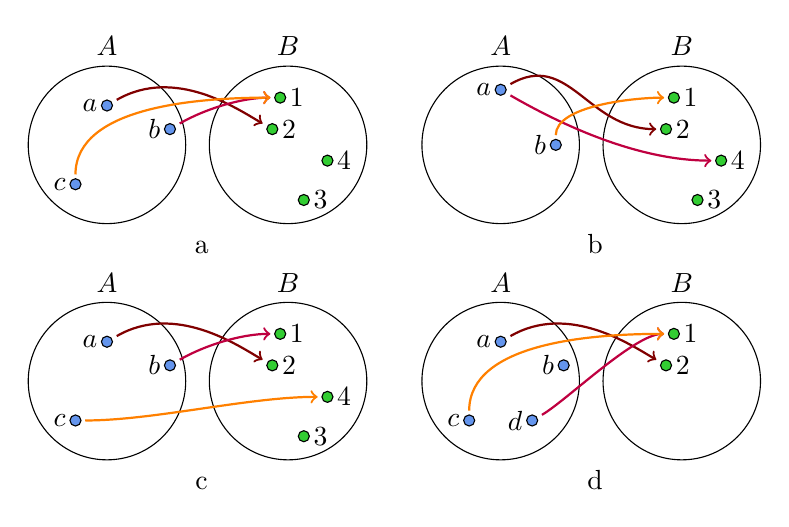
\begin{tikzpicture}[x=10mm, y=10mm]
%========================
% Prima coppia di insiemi
%========================
  \node[circle, minimum height=2cm,draw] (A) at (0,0) {};
  \node[above] (A1) at (A.north) {$A$};

  \begin{scope}[fill=CornflowerBlue]
    \filldraw (0,.5) circle (2pt) node (a) {};
    \node[left] at (0,.5) {$a$};
    \filldraw (.8,.2) circle (2pt) node (b) {};
    \node[left] at (.8,.2) {$b$};
    \filldraw (-.4,-.5) circle (2pt) node (c) {};
    \node[left] at (-.4,-.5)  {$c$};
  \end{scope}
  
  \node[anchor=south]  at (1.2,-1.5) {a};
  \begin{scope}[xshift=2.3cm]
  \node[circle, minimum height=2cm,draw] (B) at (0,0) {};
  \node[above] (B1) at (B.north) {$B$};

    \begin{scope}[fill=LimeGreen]
      \filldraw (-.1,.6) circle (2pt) node (a1) {};
      \filldraw (-.2,.2) circle (2pt)node (b1) {};
      \filldraw (.2,-.7) circle (2pt) node (c1) {};
      \filldraw(.5,-.2) circle (2pt);

      \node[right]  at (-.1,.6) {$1$};
      \node[right] at (-.2,.2) {$2$};
      \node[right]  at (.2,-.7) {$3$};
      \node[right] at (.5,-.2) {$4$};
    \end{scope}
  \end{scope}

  \begin{scope}[->,smooth,thick]
    \draw[Maroon] (a) .. controls +(30:1cm) and +(150:.5cm) .. (b1);
    \draw[purple] (b) .. controls +(30:.5cm) and +(180:0.5cm) .. (a1);
    \draw[orange] (c) .. controls +(90:1cm) and +(180:1cm) .. (a1);
  \end{scope}
%==========================
% Seconda coppia di insiemi
%==========================
  \begin{scope}[xshift=5cm]

  \node[circle, minimum height=2cm,draw] (A) at (0,0) {};
  \node[above] (A1) at (A.north) {$A$};
  \node [anchor=south] at (1.2,-1.5) {b};

  \begin{scope}[fill=CornflowerBlue]

      \filldraw (0,.7) circle (2pt) node (a) {};
      \node[left] at (0,.7) {$a$};
      \filldraw (.7,0) circle (2pt) node (b) {};
      \node[left] at (.7,0) {$b$};
    \end{scope}

    \begin{scope}[xshift=2.3cm]
      \node[circle, minimum height=2cm,draw] (B) at (0,0) {};
      \node[above] (B1) at (B.north) {$B$};

      \begin{scope}[fill=LimeGreen]
	\filldraw (-.1,.6) circle (2pt) node (a1) {};
	\filldraw (-.2,.2) circle (2pt)node (b1) {};
	\filldraw (.2,-.7) circle (2pt) node (c1) {};
	\filldraw(.5,-.2) circle (2pt) node (d1){};

	\node[right]  at (-.1,.6) {$1$};
	\node[right] at (-.2,.2) {$2$};
	\node[right]  at (.2,-.7) {$3$};
	\node[right] at (.5,-.2) {$4$};
      \end{scope}
    \end{scope}

    \begin{scope}[->,smooth,thick]
      \draw[Maroon] (a) .. controls +(30:1cm) and +(180:1cm) .. (b1);
      \draw[purple] (a) .. controls +(-30:1cm) and +(180:1cm) .. (d1);
      \draw[orange] (b) .. controls +(90:.5cm) and +(180:.5cm) .. (a1);
    \end{scope}
  \end{scope}
%========================
% Terza coppia di insiemi
%========================
  \begin{scope}[yshift=-3cm]
    \node[circle, minimum height=2cm,draw] (A) at (0,0) {};
    \node[above] (A1) at (A.north) {$A$};

    \begin{scope}[fill=CornflowerBlue]
      \filldraw (0,.5) circle (2pt) node (a) {};
      \node[left] at (0,.5) {$a$};
      \filldraw (.8,.2) circle (2pt) node (b) {};
      \node[left] at (.8,.2) {$b$};
      \filldraw (-.4,-.5) circle (2pt) node (c) {};
      \node[left] at (-.4,-.5)  {$c$};
    \end{scope}
    \node[anchor=south]  at (1.2,-1.5) {c};
    
    \begin{scope}[xshift=2.3cm]
      \node[circle, minimum height=2cm,draw] (B) at (0,0) {};
      \node[above] (B1) at (B.north) {$B$};
      
      \begin{scope}[fill=LimeGreen]
      \filldraw (-.1,.6) circle (2pt) node (a1) {};
      \filldraw (-.2,.2) circle (2pt)node (b1) {};
      \filldraw (.2,-.7) circle (2pt) node (c1) {};
      \filldraw(.5,-.2) circle (2pt) node(d1){};

      \node[right]  at (-.1,.6) {$1$};
      \node[right] at (-.2,.2) {$2$};
      \node[right]  at (.2,-.7) {$3$};
      \node[right] at (.5,-.2) {$4$};
      \end{scope}
    \end{scope}

    \begin{scope}[->,smooth,thick]
      \draw[Maroon] (a) .. controls +(30:1cm) and +(150:.5cm) .. (b1);
      \draw[purple] (b) .. controls +(30:.5cm) and +(180:0.5cm) .. (a1);
      \draw[orange] (c) .. controls +(0:1cm) and +(180:1cm) .. (d1);
    \end{scope}
  \end{scope}
%=========================  
% Quarta coppia di insiemi
%=========================  
  \begin{scope}[xshift=5cm,yshift=-3cm]
    \node[circle, minimum height=2cm,draw] (A) at (0,0) {};
    \node[above] (A1) at (A.north) {$A$};

    \begin{scope}[fill=CornflowerBlue]
      \filldraw (0,.5) circle (2pt) node (a) {};
      \node[left] at (0,.5) {$a$};
      \filldraw (.8,.2) circle (2pt) node (b) {};
      \node[left] at (.8,.2) {$b$};
      \filldraw (-.4,-.5) circle (2pt) node (c) {};
      \node[left] at (-.4,-.5)  {$c$};
      \filldraw (.4,-.5) circle (2pt) node (d) {};
      \node[left] at (.4,-.5)  {$d$};
    \end{scope}
    
    \node[anchor=south]  at (1.2,-1.5) {d};
    
    \begin{scope}[xshift=2.3cm]
    \node[circle, minimum height=2cm,draw] (B) at (0,0) {};
    \node[above] (B1) at (B.north) {$B$};

      \begin{scope}[fill=LimeGreen]
	\filldraw (-.1,.6) circle (2pt) node (a1) {};
	\filldraw (-.2,.2) circle (2pt)node (b1) {};

	\node[right]  at (-.1,.6) {$1$};
	\node[right] at (-.2,.2) {$2$};
      \end{scope}
    \end{scope}

    \begin{scope}[->,smooth,thick]
      \draw[Maroon] (a) .. controls +(30:1cm) and +(150:.5cm) .. (b1);
      \draw[purple] (d) .. controls +(30:.5cm) and +(180:0.5cm) .. (a1);
      \draw[orange] (c) .. controls +(90:1cm) and +(180:1cm) .. (a1);
    \end{scope}
  \end{scope}
\end{tikzpicture}

 \end{center}

Le corrispondenze rappresentate nelle figure~a e c sono funzioni da $A$ in $B$ poiché in tali casi tutti gli elementi del dominio $A$ hanno un corrispondente nel codominio $B$.

La corrispondenza della figura~b non rappresenta una funzione da $A$ in $B$ perché
l'elemento~$a \in A$ è in corrispondenza con due
elementi di~$B$, il~2 e il~4, quindi la corrispondenza non è univoca.
Anche la corrispondenza della figura~d non è una funzione da $A$ in $B$ perché il
dominio non coincide con l'insieme~$A$.
 \end{esempio}
\end{exrig}

I termini funzione o applicazione sono sinonimi, tuttavia si preferisce
usare il termine ``funzione'' quando i due insiemi~$A$ e~$B$ sono insiemi numerici. Solitamente una funzione
viene indicata con la lettera~$f$.
Per indicare che la funzione $f$ trasforma elementi dell'insieme~$A$ in elementi dell'insieme~$B$ usiamo una delle seguenti scritture
\begin{equation*}
f:A \rightarrow B \text{~~~oppure~~~} A\xrightarrow {f}B
\end{equation*}

\begin{definizione}\label{def:immagine_di_f}
 L'elemento~$y$ di~$B$, corrispondente di un elemento~$x$ del dominio, viene detto \emph{immagine di~$x$ nella funzione~$f$} e
si scrive~$y = f(x)$ che si legge ``$y$ uguale a effe di~$x$''.
\end{definizione}

L'insieme~$A$ si chiama~\emph{dominio}, l'insieme~$B$ \emph{codominio}.

Il sottoinsieme proprio o improprio del codominio~$B$ formato dagli elementi che sono
immagini degli elementi del dominio $\Dom$ secondo la funzione $f$ si chiama
\emph{insieme immagine} e si scrive~$\IM = f(\Dom)$. Osserviamo che non necessariamente
ogni elemento del codominio è immagine di un elemento del dominio per cui~$\IM\subseteq \Cod$.

 \vspazio\ovalbox{\risolvii \ref{ese:8.1}, \ref{ese:8.2}, \ref{ese:8.3}}

\subsection{Funzioni iniettive, suriettive, biunivoche}

\begin{exrig}
 \begin{esempio}
Nella figure sottostanti sono rappresentate alcune funzioni:
\begin{center}
 % (c) 2012 Dimitrios Vrettos - d.vrettos@gmail.com
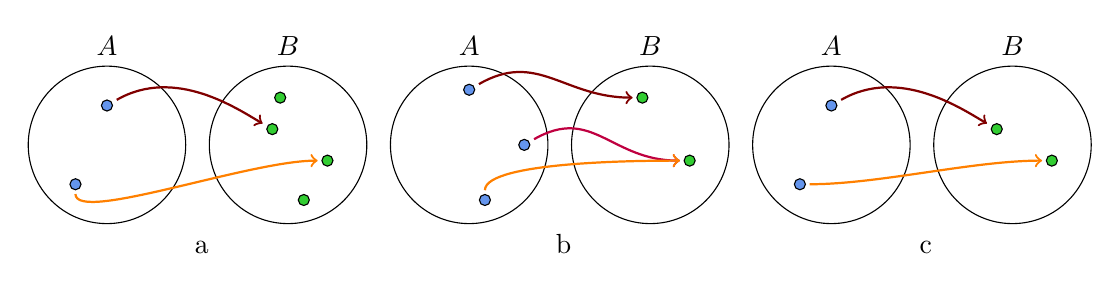
\begin{tikzpicture}[x=10mm, y=10mm]

  \node[circle, minimum height=2cm,draw] (A) at (0,0) {};
  \node[above] (A1) at (A.north) {$A$};

  \begin{scope}[fill=CornflowerBlue]
    \filldraw (0,.5) circle (2pt) node (a) {};
    \filldraw (-.4,-.5) circle (2pt) node (c) {};
    \node[left] at (-.4,-.5)  {};
  \end{scope}
  
  \node[anchor=south]  at (1.2,-1.5) {a};
  \begin{scope}[xshift=2.3cm]
    \node[circle, minimum height=2cm,draw] (B) at (0,0) {};
    \node[above] (B1) at (B.north) {$B$};
    
    \begin{scope}[fill=LimeGreen]
      \filldraw (-.1,.6) circle (2pt) node (a1) {};
      \filldraw (-.2,.2) circle (2pt)node (b1) {};
      \filldraw (.2,-.7) circle (2pt) node (c1) {};
      \filldraw(.5,-.2) circle (2pt) node(d1) {};
    \end{scope}
  \end{scope}

  \begin{scope}[->,smooth,thick]
    \draw[Maroon] (a) .. controls +(30:1cm) and +(150:.5cm) .. (b1);
    \draw[orange] (c) .. controls +(-90:.5cm) and +(180:1cm) .. (d1);
  \end{scope}

  \begin{scope}[xshift=4.6cm]
    \node[circle, minimum height=2cm,draw] (A) at (0,0) {};
    \node[above] (A1) at (A.north) {$A$};
    \node [anchor=south] at (1.2,-1.5) {b};
    \begin{scope}[fill=CornflowerBlue]

      \filldraw (0,.7) circle (2pt) node (a) {};
      \filldraw (.7,0) circle (2pt) node (b) {};
      \filldraw (.2,-.7) circle (2pt) node (c) {};
    \end{scope}

    \begin{scope}[xshift=2.3cm]
    \node[circle, minimum height=2cm,draw] (B) at (0,0) {};

    \node[above] (B1) at (B.north) {$B$};

      \begin{scope}[fill=LimeGreen]
	\filldraw (-.1,.6) circle (2pt) node (a1) {};
	\filldraw(.5,-.2) circle (2pt) node (d1){};
      \end{scope}
    \end{scope}

    \begin{scope}[->,smooth,thick]
      \draw[Maroon] (a) .. controls +(30:1cm) and +(180:1cm) .. (a1);
      \draw[purple] (b) .. controls +(30:1cm) and +(180:1cm) .. (d1);
      \draw[orange] (c) .. controls +(90:.5cm) and +(180:.5cm) .. (d1);
    \end{scope}
  \end{scope}

  \begin{scope}[xshift=9.2cm]
    \node[circle, minimum height=2cm,draw] (A) at (0,0) {};
    \node[above] (A1) at (A.north) {$A$};

    \begin{scope}[fill=CornflowerBlue]
      \filldraw (0,.5) circle (2pt) node (a) {};
      \filldraw (-.4,-.5) circle (2pt) node (c) {};
    \end{scope}
    \node[anchor=south]  at (1.2,-1.5) {c};
  
    \begin{scope}[xshift=2.3cm]
      \node[circle, minimum height=2cm,draw] (B) at (0,0) {};
      \node[above] (B1) at (B.north) {$B$};

      \begin{scope}[fill=LimeGreen]
	\filldraw (-.2,.2) circle (2pt)node (b1) {};
	\filldraw(.5,-.2) circle (2pt) node(d1){};
      \end{scope}
    \end{scope}

    \begin{scope}[->,smooth,thick]
      \draw[Maroon] (a) .. controls +(30:1cm) and +(150:.5cm) .. (b1);
      \draw[orange] (c) .. controls +(0:1cm) and +(180:1cm) .. (d1);
    \end{scope}
  \end{scope}
\end{tikzpicture}
\end{center}

Nella figura~a si ha~$\IM\subset B$: elementi distinti del dominio~$A$ hanno immagini distinte nel codominio~$B$, ma non tutti gli elementi di $B$ sono corrispondenti di un elemento di $A$.

Nella figura~b si ha~$\IM=B$ ma alcuni elementi distinti del dominio~$A$ hanno la stessa immagine nel codominio~$B$.

Nella figura~c si ha~$\IM=B$ ed elementi distinti del dominio~$A$ hanno immagini distinte nel codominio~$B$.
 \end{esempio}
\end{exrig}

I tre esempi precedenti (a, b, c) illustrano tre tipi diversi di funzioni:

\begin{definizione}
Si dice \emph{iniettiva} una funzione per la quale elementi distinti del
dominio $\Dom$ hanno immagini distinte nel codominio $\Cod$: $\forall x_1$, $x_2 \in \Dom \mid  x_1\neq x_2 \:\Rightarrow\: f(x_1)\neq f(x_2)$.
\end{definizione}

\begin{definizione}
Si dice \emph{suriettiva} una funzione per la quale~$\IM = \Cod$.
\end{definizione}

\begin{definizione}
Si dice \emph{biunivoca} o \emph{biiettiva} una funzione che sia
contemporaneamente iniettiva e suriettiva.
\end{definizione}

Pertanto nella figura~a è rappresentata una funzione iniettiva, nella figura~b una
funzione suriettiva e nella~c una funzione biunivoca.

 \vspazio\ovalbox{\risolvii \ref{ese:8.4}, \ref{ese:8.5}}
% \newpage
%\subsection{Diagramma riepilogativo sui diversi tipi di corrispondenze}
%\begin{center}
% % (c) 2012 Dimitrios Vrettos - d.vrettos@gmail.com
\begin{tikzpicture}[x=10mm, y=10mm,filled/.style={fill=circle area, thick}]
\draw (0,0) rectangle (5,4) node[above right] {$C$};
  \node[ellipse, minimum height=3cm, minimum width=4.5cm,draw=blue,thick] (F) at (2.5,2) {};
  \node[above, blue] (F1) at (F.north) {$F$};

\def\firstcircle{(1.7,1.9) circle (1cm)}
\def\secondcircle{(2.9,1.9) circle (1.25cm)}
\definecolor{circle area}{gray}{0.9}
    \begin{scope}
        \clip \firstcircle;
        \fill[filled] \secondcircle;
    \end{scope}
    \draw[OliveGreen, thick]\firstcircle;
    \draw[Maroon,thick] \secondcircle;
    \node[OliveGreen] at (1.1,1.9) {$I$};
	\node[Maroon] at (3.1,1.9) {$S$};

\begin{scope}[xshift=6cm, yshift=2cm]
\matrix[matrix of nodes, right,column 1/.style={anchor=base west,},
column 2/.style={anchor=base west}, column sep=.5cm
]{
Legenda&\\
$C$& insieme delle corrispondenze\\
|[blue]|$F$&insieme delle funzioni\\
|[Maroon]|$S$&insieme delle funzioni suriettive\\
|[OliveGreen]|$I$&insieme delle funzioni iniettive\\
$I \cap S$&insieme delle funzioni biunivoche\\};
\end{scope}
\end{tikzpicture}
%\end{center}

\section{Funzioni tra insiemi numerici}

Analizziamo alcune corrispondenze definite tra gli insiemi numerici. In
questo caso la funzione~$f$ può essere espressa
tramite una formula o scrittura analitica, una tabella, un algoritmo,
oppure semplicemente con linguaggio comune, purché in modo preciso e
inequivocabile. Il generico elemento~$x$ del dominio si chiama
\emph{variabile indipendente} e il corrispondente elemento~$y =f(x)$ si chiama \emph{variabile dipendente}.

\begin{exrig}
 \begin{esempio}
 \label{ex:8.3}
Consideriamo la corrispondenza~$\Kor$: ``essere il valore assoluto di'' tra l'insieme~$\insN_0$ dei naturali diversi da zero e l'insieme~$\insZ_0$ degli interi
relativi diversi da zero.

Questa corrispondenza non è una
funzione in quanto non è una corrispondenza univoca: ogni elemento di~$\insN_0$ ha due immagini
poiché ogni numero naturale è valore assoluto di due interi
opposti, come rappresentato dalla figura~\ref{fig:8.1}.
\end{esempio}

\begin{figure}[b]
 \begin{minipage}[t]{.45\textwidth}
\centering
 % (c) 2012 Dimitrios Vrettos - d.vrettos@gmail.com
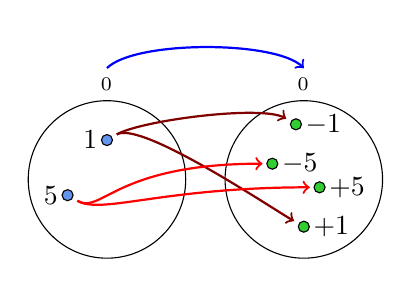
\begin{tikzpicture}[x=10mm, y=10mm]

\node[circle, minimum height=2cm,draw] (D) at (0,0) {};

\node[above] (D1) at (D.north) {$\insN_0$};
\begin{scope}[fill=CornflowerBlue]

\filldraw (0,.5) circle (2pt) node (a) {};
\node[left] at (0,.5) {1};
\filldraw (-.5,-.2) circle (2pt) node (d) {};
\node[left] at (-.5,-.2) {5};
\end{scope}

\begin{scope}[xshift=2.5cm]
\node[circle, minimum height=2cm,draw] (C) at (0,0) {};

\node[above] (C1) at (C.north) {$\insZ_0$};

\begin{scope}[fill=LimeGreen]
\filldraw (-.1,.7) circle (2pt) node (a1) {};
\filldraw (-.4,.2) circle (2pt)node (b1) {};
\filldraw (0,-.6) circle (2pt) node (c1) {};
\filldraw (.2,-.1) circle (2pt) node (d1) {};
\node[right]  at (-.1,.7) {$-1$};
\node[right]  at (0,-.6) {$+1$};
\node[right] at (-.4,.2) {$-5$};
\node[right] at (.2,-.1) {$+5$};
\end{scope}
\end{scope}
\begin{scope}[->,smooth,thick]
\draw[blue] (D1.north) .. controls +(45:.5cm) and +(135:.5cm) .. (C1.north) node [midway, above, black] () {$\Kor$};
\draw[Maroon] (a) .. controls +(30:.5cm) and +(150:.5cm) .. (c1);
 \draw[Maroon] (a) .. controls +(30:.5cm) and +(150:.5cm) .. (a1);
\draw[red] (d) .. controls +(-30:.5cm) and +(-180:2cm) .. (b1);
\draw[red] (d) .. controls +(-30:.5cm) and +(-180:2cm) .. (d1);
\end{scope}
\end{tikzpicture}

\caption{}\label{fig:8.1}
 \end{minipage}\hfil
 \begin{minipage}[t]{.45\textwidth}
\centering
 % (c) 2012 Dimitrios Vrettos - d.vrettos@gmail.com
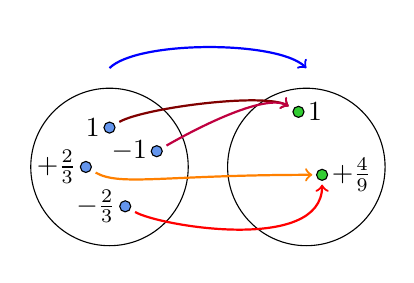
\begin{tikzpicture}[x=10mm, y=10mm]

\node[circle, minimum height=2cm,draw] (D) at (0,0) {};

\node[above] (D1) at (D.north) {$\insQ$};
\begin{scope}[fill=CornflowerBlue]

\filldraw (0,.5) circle (2pt) node (a) {};
\node[left] at (0,.5) {1};
\filldraw (0.6,.2) circle (2pt) node (b) {};
\node[left] at (0.6,.2) {$-1$};
\filldraw (.2,-.5) circle (2pt) node (c) {};
\node[left] at (.2,-.5) {$-\frac{2}{3}$};
\filldraw (-.3,0) circle (2pt) node (d) {};
\node[left] at (-.3,0) {$+\frac{2}{3}$};
\end{scope}

\begin{scope}[xshift=2.5cm]
\node[circle, minimum height=2cm,draw] (C) at (0,0) {};

\node[above] (C1) at (C.north) {$\insQ$};

\begin{scope}[fill=LimeGreen]
\filldraw (-.1,.7) circle (2pt) node (a1) {};
\filldraw (.2,-.1) circle (2pt) node (d1) {};
\node[right]  at (-.1,.7) {$1$};
\node[right] at (.2,-.1) {$+\frac{4}{9}$};
\end{scope}
\end{scope}
\begin{scope}[->,smooth,thick]
\draw[blue] (D1.north) .. controls +(45:.5cm) and +(135:.5cm) .. (C1.north) node [midway, above, black] () {$\Kor$};
\draw[Maroon] (a) .. controls +(30:.5cm) and +(150:.5cm) .. (a1);
 \draw[purple] (b) .. controls +(30:.5cm) and +(150:.5cm) .. (a1);
\draw[red] (c) .. controls +(-30:.5cm) and +(-90:1cm) .. (d1);
\draw[orange] (d) .. controls +(-30:.5cm) and +(-180:2cm) .. (d1);
\end{scope}
\end{tikzpicture}
\caption{}\label{fig:8.2}
 \end{minipage}
\end{figure}

 \begin{esempio}
 \label{ex:8.4}
 Consideriamo la corrispondenza~$\Kor$ che associa ad ogni numero razionale il suo quadrato.

Essa è una funzione di
dominio~$\insQ$ e codominio $\insQ$: di ogni numero razionale si può
determinare il quadrato che è unico; poiché numeri opposti hanno lo
stesso quadrato la funzione in esame \emph{non} è
\emph{iniettiva}, come rappresentato dalla figura~\ref{fig:8.2}.

L'immagine~$y$ di ogni~$x$ appartenente a~$\insQ$ è il suo
quadrato: in simboli matematici scriviamo la funzione tramite una
formula~$f: y = x^{2}$.

Per quanto riguarda l'insieme immagine
della funzione esso è un sottoinsieme proprio di~$\insQ$: ad esempio, il numero razionale~$+{\frac{3}{4}}$ non è quadrato di
nessun razionale e neppure~$-25$, razionale negativo, è quadrato di
un numero razionale, quindi~$\IM\subset\insQ^{+}\cup\{0\}$, pertanto la funzione da $\insQ$ in $\insQ$ non è suriettiva.
 \end{esempio}

 \begin{esempio}
 \label{ex:8.5}
 Analizziamo la corrispondenza che associa ad ogni intero il suo valore assoluto.

Sappiamo che il valore assoluto di un intero è un numero naturale, e
ogni intero ha un solo valore assoluto. La corrispondenza è univoca e
il dominio coincide con l'insieme~$\insZ$, pertanto è una
funzione:~$f: \insZ\rightarrow\insN$ che è rappresentata in forma
analitica con la scrittura~${y=\valass{x}}$ con~$x\in\insZ$ e~$y=f(x)\in\insN$.

\begin{center}
\begin{tabular}{l*8{c}}
 \toprule
$x\in \insZ$ & 0 & $+1$ & $-1$ & $-2$ & $+2$ & $+3$ & $-3$ & \ldots\\
$y\in \insN$ & 0 & 1 & 1 & 2 & 2 & 3 & 3 & \ldots \\
\bottomrule
\end{tabular}
\end{center}
Nella tabella sono rappresentati alcuni elementi del dominio
con le rispettive immagini: da cui si deduce che tale funzione non è
iniettiva.
 \end{esempio}

 \begin{esempio}
 \label{ex:8.6}
È assegnata la funzione~$f:x\in \insN\rightarrow (x-2)\in\insZ$. In questo caso la funzione associa ad ogni numero naturale $x$ il
numero intero ottenuto sottraendogli~2. L'espressione analitica della funzione $f$ è: $y = x-2$. La legge così espressa si può descrivere anche attraverso una
tabella.

\begin{center}
\begin{tabular}{l*8{c}}
 \toprule
$x\in \insN$ & 0 & 1 & 2 & 3 & 4 & 5 & 6 & \ldots \\
$(x-2)\in \insZ$ & $-2$ & $-1$ & 0 & $+1$ & $+2$ & $+3$ & $+4$ & \ldots \\
\bottomrule
\end{tabular}
\end{center}

Ogni elemento dell'insieme~$\insN$ trova il corrispondente in~$\insZ$; elementi diversi del dominio hanno immagini diverse pertanto la
funzione è \emph{iniettiva}; l'insieme immagine è un sottoinsieme proprio del codominio~$\insZ$ e precisamente~$IM =\{y\in\insZ\mid y\ge -2\} \subset \insZ$,
pertanto la funzione da $\insN$ a $\insZ$ non è suriettiva.
 \end{esempio}

 \begin{esempio}
 \label{ex:8.7}
 Analizziamo la corrispondenza:~$f_{1}:x\in \insN\rightarrow (x-2)\in \insN$ e costruiamo la relativa tabella:

\begin{center}
\begin{tabular}{l*8{c}}
\toprule
$x\in \insN$ & 0 & 1 & 2 & 3 & 4 & 5 & 6 & \ldots \\
$(x-2)\in \insN$ & & & 0 & 1 & 2 & 3 & 4 & \ldots \\
\bottomrule
\end{tabular}
\end{center}
Vediamo che nella corrispondenza assegnata né~0 né~1 hanno l'immagine in $\insN$.

Fissiamo allora come dominio $\Dom$ un sottoinsieme di~$\insN$ e precisamente~$\Dom = \ID = \insN - \{$0, 1$\}$;
in questo modo possiamo procedere nell'analisi della funzione~$f_{1}:y=x-2$.
\end{esempio}

\begin{esempio}
 Consideriamo la corrispondenza che associa ad ogni numero razionale il suo inverso (o reciproco).

Sappiamo che ``fare l'inverso'' di un numero razionale~$x$
significa scrivere il numero razionale~$\frac{1}{x}$, ma questa
operazione ha significato solo se~$x$ è diverso da~0; operiamo dunque
una restrizione su $\insQ$ e fissiamo~$\Dom = \ID = \insQ_0$. La corrispondenza è una funzione $f: y=\frac{1}{x}$ da~$\insQ_0$ in~$\insQ$.
 \end{esempio}
\end{exrig}


\ovalbox{\risolvii \ref{ese:8.6}, \ref{ese:8.7}, \ref{ese:8.8}, \ref{ese:8.9}, \ref{ese:8.10}, \ref{ese:8.11}}

\subsection{Funzioni inverse}

\`E assegnata la funzione~$f:\insR\rightarrow \insR$ descritta mediante le istruzioni
\begin{center}
 % (c) 2012 Dimitrios Vrettos - d.vrettos@gmail.com
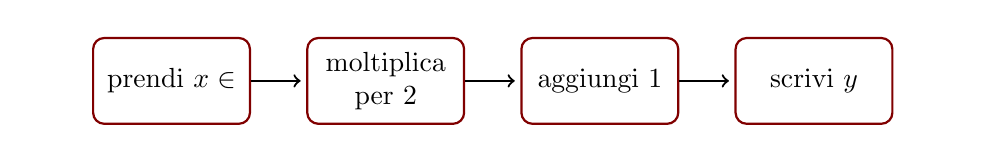
\begin{tikzpicture}
[auto,block/.style
={rectangle, draw=Maroon, thick,
text width=5em,align=center, rounded corners,
minimum height=3.1em},
line/.style
={draw, thick, ->,shorten >=2pt}]
\matrix [column sep=7mm]{
& \node [block] (prn) {prendi $x\in \insR$}; 
& \node [block] (molt) {moltiplica per 2}; 
& \node [block] (agg) {aggiungi 1}; 
& \node [block] (scr) {scrivi $y$}; & \\
};
\begin{scope}[every path/.style=line]
\path (prn)-- (molt);
\path (molt) -- (agg);
\path (agg)--(scr);
\end{scope}
\end{tikzpicture}
\end{center}

La forma algebrica è~$y=2\cdot x+1$; essa è definita per qualunque
numero reale, quindi $\Dom = \insR$ e l'insieme immagine coincide con il codominio, $\IM=\Cod=\insR$.
Scelto arbitrariamente un valore per la variabile
indipendente come~$x=-2$ otteniamo la sua immagine~$y=f(-2)=-3$, risultato
delle operazioni descritte nelle istruzioni.

Preso ora~$y=4$, elemento dell'insieme immagine della
funzione, quali istruzioni dobbiamo seguire per determinarne la
controimmagine? Cioè di quale elemento di $\Dom$ è immagine il valore~4?
Per quale valore di~$x$ aggiungendo~1 al suo doppio si
ottiene~4?
La questione è rappresentata nel diagramma di Eulero-Venn della figura~\ref{fig:8.3} e
percorrendo le istruzioni con le operazioni inverse otteniamo il valore di~$x$
sottraendo~1 al valore dato per~$y$ e dividendo il risultato per~2. Le
istruzioni da eseguire per determinare la controimmagine sono quindi:
\begin{center}
 % (c) 2012 Dimitrios Vrettos - d.vrettos@gmail.com
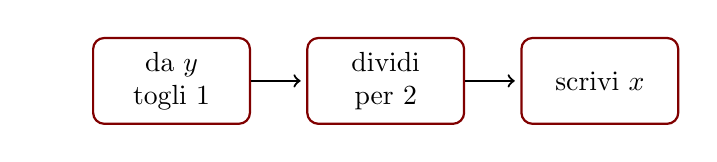
\begin{tikzpicture}
[auto,block/.style
={rectangle, draw=Maroon, thick,
text width=5em,align=center, rounded corners,
minimum height=3.1em},
line/.style
={draw, thick, ->,shorten >=2pt}]
\matrix [column sep=7mm]{
& \node [block] (prn) { da~$y$ togli 1}; 
& \node [block] (molt) {dividi per 2}; 
& \node [block] (agg) {scrivi~$x$}; \\
};
\begin{scope}[every path/.style=line]
\path (prn)-- (molt);
\path (molt) -- (agg);
\end{scope}
\end{tikzpicture}
\end{center}
In formula~$x=(y-1):2$.
La funzione così ottenuta si chiama \emph{funzione inversa} di~$f(x)$, che è quella che dato un elemento di $\IM$ ci fornisce l'elemento di $\Dom$ di cui è l'immagine.
Questo è possibile poiché la funzione assegnata è iniettiva, e pertanto ci rendiamo subito conto che è invertibile, cioè che per ogni~$y\in\IM$ possiamo determinare la sua controimmagine $x\in\Dom$.

\begin{figure}[h,b]
\centering% (c) 2012 Dimitrios Vrettos - d.vrettos@gmail.com
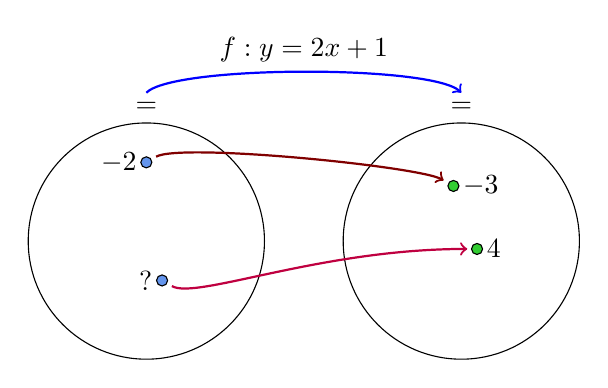
\begin{tikzpicture}[x=10mm, y=10mm]

\node[circle, minimum height=3cm,draw] (D) at (0,0) {};

\node[above] (D1) at (D.north) {$\Dom=\insR$};
\begin{scope}[fill=CornflowerBlue]

\filldraw (0,1) circle (2pt) node (a) {};
\node[left] at (0,1) {$-2$};

\filldraw (.2,-.5) circle (2pt) node (c) {};
\node[left] at (.2,-.5) {?};

\end{scope}

\begin{scope}[xshift=4cm]
\node[circle, minimum height=3cm,draw] (C) at (0,0) {};

\node[above] (C1) at (C.north) {$\Cod=\insR$};

\begin{scope}[fill=LimeGreen]
\filldraw (-.1,.7) circle (2pt) node (a1) {};
\filldraw (.2,-.1) circle (2pt) node (d1) {};
\node[right]  at (-.1,.7) {$-3$};
\node[right] at (.2,-.1) {$4$};
\end{scope}
\end{scope}
\begin{scope}[->,smooth,thick]
\draw[blue] (D1.north) .. controls +(45:.5cm) and +(135:.5cm) .. (C1.north) node [midway, above, black] () {$f:y=2x+1$};
\draw[Maroon] (a) .. controls +(30:.5cm) and +(150:.5cm) .. (a1);
\draw[purple] (c) .. controls +(-30:.5cm) and +(-180:2cm) .. (d1);
\end{scope}
\end{tikzpicture}
\caption{Funzioni inverse.}\label{fig:8.3}
\end{figure}

\begin{definizione}\label{def:funzione_inversa}
Data una funzione iniettiva~$f:\Dom \rightarrow \Cod$ tale che $y = f(x)$ si definisce la sua \emph{funzione inversa} $f^{-1}:\IM \rightarrow \Dom$ come quella che permette di determinare la
controimmagine di un qualunque elemento di $\IM$, ovvero $x = f^{-1}(y)$.
\end{definizione}

Osserviamo che~$\Dom\left(f^{-1}\right)=\IM(f)$ e~$\IM\left(f^{-1}\right)=\Dom(f)$.

\vspazio\ovalbox{\risolvi \ref{ese:8.12}}

\section{Funzioni composte}

\begin{definizione}
Date due funzioni~$f:A\rightarrow B$ e~$g:B\rightarrow C$ si
definisce la \emph{funzione composta}
\[g\circ f:A\rightarrow C\]
una funzione che a un elemento~$a \in A$ associa prima l'elemento~$b=f(a)\in B$ e
poi l'elemento~$c=g(b) \in C$. In un'unica
formula si può scrivere~$g(f(a))=c$.
\end{definizione}
\pagebreak
\begin{exrig}
 \begin{esempio}
 Data la funzione~$f(x)=2x$ e la funzione~$g(x)=x^2+1$, determina
l'espressione analitica della funzione composta.

Prima agisce la funzione~$f$ che raddoppia il valore di~$x$. Al valore
così ottenuto, che è~$2x$, si applica la~$g$ che lo eleva al quadrato
e gli aggiunge~1. Pertanto
la funzione composta quadruplica il quadrato di~$x$ e poi aggiunge~1.
L'espressione è~$g(f(x))=(2x)^2+1 = 4x^2+1$.
 \end{esempio}

\begin{center}
 % (c) 2012 Dimitrios Vrettos - d.vrettos@gmail.com
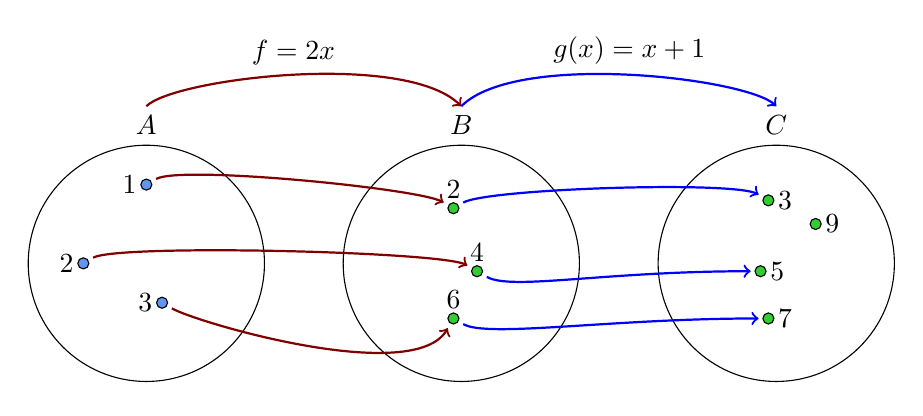
\begin{tikzpicture}[x=10mm, y=10mm]

\node[circle, minimum height=3cm,draw] (A) at (0,0) {};

\node[above] (A1) at (A.north) {$A$};
\begin{scope}[fill=CornflowerBlue]

\filldraw (0,1) circle (2pt) node (a) {};
\node[left] at (0,1) {$1$};
\filldraw (-.8,0) circle (2pt) node (b) {};
\node[left] at (-.8,0) {$2$};
\filldraw (.2,-.5) circle (2pt) node (c) {};
\node[left] at (.2,-.5) {$3$};

\end{scope}

\begin{scope}[xshift=4cm]
\node[circle, minimum height=3cm,draw] (B) at (0,0) {};

\node[above] (B1) at (B.north) {$B$};

\begin{scope}[fill=LimeGreen]
\filldraw (-.1,.7) circle (2pt) node (a1) {};
\filldraw (-.1,-.7) circle (2pt) node (c1) {};
\filldraw (.2,-.1) circle (2pt) node (b1) {};
\node[above]  at (-.1,.7) {$2$};
\node[above] at (.2,-.1) {$4$};
\node[above]  at (-.1,-.7) {$6$};
\end{scope}
\end{scope}
\begin{scope}[->,smooth,thick]
\draw[Maroon] (A1.north) .. controls +(45:.5cm) and +(135:1cm) .. (B1.north) node [midway, above, black] () {$f=2x$};
\draw[Maroon] (a) .. controls +(30:.5cm) and +(150:.5cm) .. (a1);
\draw[Maroon] (b) .. controls +(30:.5cm) and +(150:.5cm) .. (b1);
\draw[Maroon] (c) .. controls +(-30:.5cm) and +(-120:1cm) .. (c1);
\end{scope}

\begin{scope}[xshift=8cm]
\node[circle, minimum height=3cm,draw] (C) at (0,0) {};

\node[above] (C1) at (C.north) {$C$};

\begin{scope}[fill=LimeGreen]
\filldraw (-.1,.8) circle (2pt) node (a2) {};
\filldraw (-.1,-.7) circle (2pt) node (c2) {};
\filldraw (-.2,-.1) circle (2pt) node (b2) {};
\filldraw (.5,.5) circle (2pt) node (d2) {};
\node[right]  at (-.1,.8) {$3$};
\node[right] at (-.2,-.1) {$5$};
\node[right]  at (-.1,-.7) {$7$};
\node[right]  at (.5,.5) {$9$};
\end{scope}
\end{scope}
\begin{scope}[->,smooth,thick]
 \draw[blue] (B1.north) .. controls +(45:1cm) and +(135:.5cm) .. (C1.north) node [midway, above, black] () {$g(x)=x+1$};
\draw[blue] (a1) .. controls +(30:.5cm) and +(150:.5cm) .. (a2);
\draw[blue] (b1) .. controls +(-30:.5cm) and +(-180:2cm) .. (b2);
\draw[blue] (c1) .. controls +(-30:.5cm) and +(-180:2cm) .. (c2);
\end{scope}
\end{tikzpicture}
\end{center}

\end{exrig}

Osserva che la composizione di funzioni non è commutativa. Infatti, nell'esempio precedente, la
funzione~$f(g(x))$ si ottiene facendo agire prima la~$g(x)$ che eleva
al quadrato il valore della variabile e lo aumenta di~1
e poi la~$f(x)$ che raddoppia il valore di quanto ottenuto;
allora~$f(g(x))=2(x^2+1)=2x^2+2$.

\vspazio\ovalbox{\risolvii \ref{ese:8.13}, \ref{ese:8.14}, \ref{ese:8.15}, \ref{ese:8.16}}

\section{La retta e gli insiemi numerici}

Nello studio degli insiemi numerici abbiamo visto come si possono depositare su una semiretta i numeri naturali;
la legge costruttiva di questa rappresentazione genera tra l'insieme~$\insN=\{$0, 1, 2, 3, 4, \ldots$\}$ e i punti della
semiretta una corrispondenza avente come dominio~$\insN$ e come codominio i punti della semiretta.
Ad ogni numero naturale possiamo far corrispondere un punto della semiretta, ma non tutti i punti della semiretta
sono immagine di un numero naturale: la corrispondenza non è biunivoca.

Lo stesso fatto avviene se consideriamo l'insieme~$\insZ$ come dominio e i punti di una retta orientata come codominio;
nella figura seguente viene rappresentata la corrispondenza generata con la legge costruttiva già enunciata nel capitolo dei numeri interi $\insZ$.
\begin{center}
 % (c) 2012 Dimitrios Vrettos - d.vrettos@gmail.com
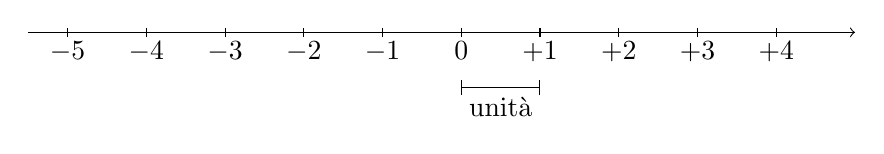
\begin{tikzpicture}[x=10mm, y=10mm]
\draw[->](-5.5,0) -- (5,0);
\foreach \x in {-5,-4,...,4}
\draw (\x,1.5pt) -- (\x,-1.5pt);

\draw[|-|] (0,-.7) -- (1,-.7) node [below, midway] () {unità};

\foreach \x/\xtext in {-5/-5,-4/-4,-3/-3,-2/-2,-1/-1,0/0,1/+1,2/+2,3/+3,4/+4}
\node[below] at (\x,0) {$\xtext$};
\end{tikzpicture}
\end{center}
Ad ogni numero intero possiamo far corrispondere un punto della retta orientata, ma non tutti i punti della retta sono immagine
di un numero intero: l'insieme immagine non coincide con il codominio e la corrispondenza non è biunivoca.

Gli insiemi~$\insN$ e~$\insZ$ sono infiniti e la loro caratteristica comune è che tra due naturali consecutivi o tra due interi consecutivi
non possiamo trovarne un altro. Si dice che~$\insN$ e~$\insZ$ sono due \emph{insiemi discreti}.

Consideriamo ora l'insieme~$\insQ$ dei numeri razionali; sappiamo che anche questi numeri, rappresentati da frazioni, possono essere disposti
su una retta orientata come mostrato nella figura sottostante.
\begin{center}
 % (c) 2012 Dimitrios Vrettos - d.vrettos@gmail.com
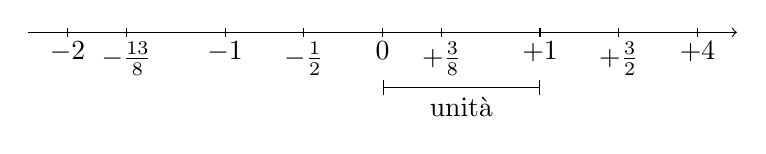
\begin{tikzpicture}[x=10mm, y=10mm]
\draw[->](-4.5,0) -- (4.5,0);
\foreach \x in {-4,-3.25,-2,-1,0,.75,2,3,4}
\draw (\x,1.5pt) -- (\x,-1.5pt);

\draw [|-|](0,-.7) -- (2,-.7) node [below, midway] () {unità};

\foreach \x/\xtext in {-4/-2,-3.25/-\frac{13}{8},-2/-1,-1/-\frac{1}{2},0/0,.75/+\frac{3}{8},2/+1,3/+\frac{3}{2},4/+4}
\node[below] at (\x,0) {$\xtext$};
\end{tikzpicture}
\end{center}
L'insieme~$\insQ$ rispetto agli insiemi~$\insN$ e~$\insZ$ presenta un'altra caratteristica: è \emph{denso}, cioè tra due numeri razionali
ci sono infiniti altri numeri razionali.
Come possiamo confermare questa affermazione?

Osserviamo la figura precedente: fra~$\frac{3}{8}$ e~$\frac{3}{2}$ si trova certamente il numero~$1$.
Costruiamo il numero~$q=\frac{1}{2} \cdot \left(\frac{3}{8}+\frac{3}{2}\right)$ ottenuto dividendo per due la somma dei due numeri estremi
dell'intervallo considerato, si ottiene~$q=\frac{15}{16}$ che è minore di~$1$ e, a maggior ragione, minore di~$\frac{3}{2}$,
ma maggiore di~$\frac{3}{8}$, come si può verificare trasformando la frazione in una equivalente con denominatore~$16$.
Con lo stesso procedimento possiamo determinare~$q_{1}=\frac{1}{2}\cdot \left(\frac{3}{8}+\frac{15}{16}\right)=\frac{21}{32}$
che risulta maggiore di~$\frac{3}{8}$ e minore di~$q$. Con questo procedimento, che non ha mai termine, possiamo determinare
infiniti altri numeri razionali compresi tra~$\frac{3}{8}$ e~$\frac{3}{2}$.
\begin{center}
 % (c) 2012 Dimitrios Vrettos - d.vrettos@gmail.com
\begin{tikzpicture}[x=10mm, y=10mm]
\draw[->](-4.5,0) -- (4.5,0);
\foreach \x in {-4,-1.93,-1.03,4}
\draw (\x,1.5pt) -- (\x,-1.5pt);

\foreach \x/\xtext in {-4/\frac{3}{8},-1.93/\frac{21}{32},-1.03/\frac{15}{16},4/\frac{3}{2}}
\node[below] at (\x,0) {$\xtext$};
\end{tikzpicture}
\end{center}

Questa possibilità ci fa supporre che tutti i punti della retta orientata possano essere immagine di un numero razionale,
cioè che esista una corrispondenza biunivoca tra l'insieme~$\insQ$ e i punti della retta.
Invece, no!
%Nella sezione~\ref{sect:intro_numeri_reali} a pagina~\pageref{sect:intro_numeri_reali}, abbiamo visto che 
Benché l'insieme~$\insQ$ sia infinito e denso,
quando pensiamo di aver disposto sulla retta tutti i suoi elementi su quest'ultima rimangono ancora altri punti liberi (es.~$\sqrt{2}$).
La retta geometrica sembra avere ``più punti'' di quanti siano i numeri razionali: gli infiniti punti lasciati scoperti dai razionali
sono immagine di numeri irrazionali $\insJ$.

L'insieme $\insR = \insQ \cup \insJ$ è l'insieme dei numeri reali, cui
Cantor attribuì la cardinalità (o potenza) del \emph{continuo}~$\aleph_1$ (superiore a quella \emph{numerabile} dei numeri naturali~$\aleph_0$).
%\footnote{si veda anche la sezione~\ref{sect:insiemi_finiti_e_infiniti} a pagina~\pageref{sect:insiemi_finiti_e_infiniti}.}
La retta geometrica orientata è in corrispondenza biunivoca con~$\insR$,
quindi ad ogni numero reale corrisponde un punto sulla retta orientata e un punto della retta è immagine
di un solo numero reale (razionale o irrazionale).

\begin{definizione}
Si chiama \emph{ascissa di un punto} sulla retta reale il numero reale~$\alpha$ che è la sua immagine nella corrispondenza biunivoca.
\end{definizione}
%\pagebreak

%\begin{exrig}
% \begin{esempio}
%Determinare l'immagine del numero reale~$\alpha =1+\sqrt{2}$ sulla retta reale.

%Fisso la retta orientata e un suo punto~$O$ al quale attribuisco ascissa~$0$;
%fisso un segmento arbitrario come unità di misura e quindi determino il punto~$A$ di ascissa~$1$ riportando il segmento unitario
%a partire da~$O$, nel verso indicato dalla freccia.
%\begin{center}
% % (c) 2012 Dimitrios Vrettos - d.vrettos@gmail.com
\begin{tikzpicture}[x=10mm, y=10mm]
\draw[->](-4.5,0) -- (4.55,0);
\foreach \x in {-2.5,0}
\draw (\x,1.5pt) -- (\x,-1.5pt);

\draw [|-|](-2.5,-.7) -- (0,-.7) node [below, midway] () {unità};
\draw [orange,thick](-2.5,0) -- (0,0);
\foreach \x/\xtext in {-2.5/0,0/1}
\node[below] at (\x,0) {$\xtext$};
\node[above] at(-2.5,0) {$O$};
\node[above] at(0,0) {$A$};
\end{tikzpicture}
%\end{center}
%Costruisco il segmento rappresentativo del numero irrazionale~$\sqrt{2}$, che, per il teorema di Pitagora, è la diagonale del quadrato di lato 1.
%Metto questo segmento adiacente al segmento~$OA$, come in figura.
%Il punto~$B$ è l'immagine del numero~$\alpha$, scriviamo~$B(\alpha)$.
%\begin{center}
% % (c) 2012 Dimitrios Vrettos - d.vrettos@gmail.com
\begin{tikzpicture}[x=10mm, y=10mm]
\draw[->](-3.5,0) -- (4.55,0);
\foreach \x in {-2.5,0,3.6}
\draw (\x,1.5pt) -- (\x,-1.5pt);

\draw [orange,thick](-2.5,0) -- (0,0);
\draw [CornflowerBlue,thick](3.6,0) -- (0,0);

\foreach \x/\xtext in {-2.5/0,0/1,3.6/\alpha}
\node[below] at (\x,0) {$\xtext$};
\node[above] at(-2.5,0) {$O$};
\node[above] at(0,0) {$A$};
\node[above] at(3.6,0) {$B$};

\begin{scope}[shift={(5,-1.25)}]
\draw (0,0) rectangle  (2.5,2.5);
\draw[CornflowerBlue,thick] (0,0) --  (2.5,2.5);
\end{scope}
\end{tikzpicture}

%\end{center}
% \end{esempio}
%\end{exrig}

%\subsubsection*{Sulla retta razionale si possono collocare tutti i numeri del tipo~$\sqrt{n}$ con~$n\in \insN_{0}$.}

%Nella figura è segnato il punto~$K$ immagine del numero~$\sqrt{2}$; sulla perpendicolare alla retta~$r$ nel punto~$K$
%prendiamo il segmento~$KD=OA$ e congiungiamo~$D$ con~$O$. Per il teorema di Pitagora sul
%triangolo~$OKD$ si ha
%\[\overline{OD}^{2}=\overline{OK}^{2}+\overline{KD}^{2}=\overline{OK}^{2}+\overline{OA}^{2}\]
%e passando alle misure
\[\overline{OD}^{2}=(\sqrt{2})^{2}+1^{2}=2+1=3\Rightarrow\overline{OD}=\sqrt{3}.\]
%Puntando il compasso in~$O$ con raggio~${OD}$ tracciamo l'arco che incontra la retta~$r$ in~$H$ immagine
%del numero irrazionale~${\sqrt{3}}$.
%\begin{center}
% % (c) 2012 Dimitrios Vrettos - d.vrettos@gmail.com
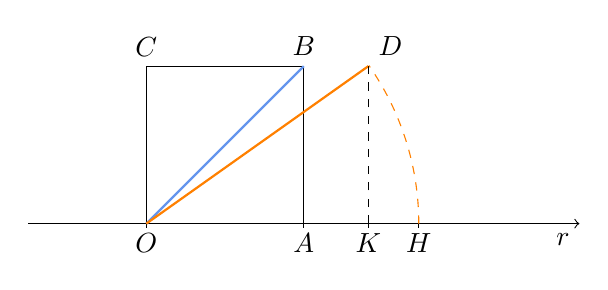
\begin{tikzpicture}[x=10mm, y=10mm]
\draw[->](-3.5,0) -- (3.5,0) node [below left] {$r$};
\foreach \x in {-2,0,.82,1.46}
\draw (\x,1.5pt) -- (\x,-1.5pt);

\foreach \x/\xtext in {-2/O,0/A,0.82/K,1.46/H}
\node[below] at (\x,0) {$\xtext$};

\draw (-2,0) rectangle  (0,2);
\draw[CornflowerBlue,thick] (-2,0) --  (0,2) node[above, black] {$B$};
\draw[orange,thick] (-2,0) --  (0.82,2) node[above right, black] {$D$};
\draw[dashed] (.82,0) -- (.82,2);
   \draw[dashed,orange] (1.46,0) arc [start angle=0, end angle=35,radius=3.5cm];

\node [above] at (-2,2) {$C$};
\end{tikzpicture}
%\end{center}
%Proseguendo in questo modo possiamo ottenere sulla retta razionale i punti associati ai numeri del tipo~${\sqrt{n}}$.

%Un'altra classica costruzione, nota come ``spirale di Teodoro'' (figura~\ref{fig:8.4}), permette di ottenere i segmenti di misura~$\sqrt{n}$ con~$n\in \insN_{0}$.
%Si inizia con la costruzione del triangolo rettangolo isoscele $OAB$ di cateto~$1$; sappiamo già che la sua ipotenusa $OB$ è il segmento
%di misura~$\sqrt{2}$. Sulla perpendicolare in~$B$ a~$OB$ si prende il segmento~$BC$ di misura~$1$:
%applicando il teorema di Pitagora al triangolo rettangolo $OBC$, come abbiamo fatto sopra, otteniamo~$\overline{OC}=\sqrt{3}$.
%Ripetiamo la costruzione dal vertice~$D$ e otteniamo il triangolo rettangolo~$OCD$ la cui ipotenusa è~$\overline{OD}=\sqrt{4}$
%e poi~$\overline{OE}=\sqrt{5}$ e così via.
%\begin{figure}[t]
% \centering% (c) 2012 Dimitrios Vrettos - d.vrettos@gmail.com
\begin{tikzpicture}[x=10mm, y=10mm]
  \tkzDefPoint(0,0){O}
  \tkzDefPoint(2,0){A}
  \tkzDefPoint(2,2){B}

  \tkzDrawPolygon(O,A,B)

  \tkzDrawTriangle[two angles=35.26 and 90](O,B) 
  \tkzGetPoint{C}

  \tkzDrawTriangle[two angles=30 and 90](O,C) 
  \tkzGetPoint{D}

  \tkzDrawTriangle[two angles=26.57 and 90](O,D) 
  \tkzGetPoint{E}

  \tkzDrawTriangle[two angles=24.1 and 90](O,E) 
  \tkzGetPoint{F}

  \tkzDrawTriangle[two angles=22.21 and 90](O,F) 
  \tkzGetPoint{G}

  \tkzLabelPoints[below](O)
  \tkzLabelPoints[right](A,B)
  \tkzLabelPoints[above](C,D,E)
  \tkzLabelPoints[left](F,G)

  \tkzMarkRightAngles[draw=Maroon](O,A,B O,B,C O,C,D O,D,E O,E,F O,F,G)

  \tkzLabelSegment[right](A,B){$1$}
  \tkzLabelSegment[above right](B,C){$1$}
  \tkzLabelSegment[above](C,D){$1$}
  \tkzLabelSegment[above](D,E){$1$}
  \tkzLabelSegment[above left](E,F){$1$}
  \tkzLabelSegment[left](F,G){$1$}

  \tkzLabelSegment[above](O,A){$\sqrt{1}$}
  \tkzLabelSegment[above=4pt](O,B){$\sqrt{2}$}
  \tkzLabelSegment[above left](O,C){$\sqrt{3}$}
  \tkzLabelSegment[above left=6pt](O,D){$\sqrt{4}$}
  \tkzLabelSegment[left=6pt](O,E){$\sqrt{5}$}
  \tkzLabelSegment[below](O,F){$\sqrt{6}$}
  \tkzLabelSegment[below](O,G){$\sqrt{7}$}
\end{tikzpicture}\vspace{-15ex}
% \caption{La spirale di Teodoro.}\label{fig:8.4}
%\end{figure}

\vspazio\ovalbox{\risolvii \ref{ese:8.17}, \ref{ese:8.18}, \ref{ese:8.19}}

\section{Il metodo delle coordinate cartesiane}\label{sect:coordinate_cartesiane}

Abbiamo definito prodotto cartesiano di due insiemi non vuoti~$A$ e~$B$ l'insieme formato da tutte
le coppie ordinate tali che il primo elemento appartenga ad~$A$ e il secondo a~$B$. Mediante proprietà caratteristica
si scrive:~$A\times B=\{(a;b)\mid a\in A\text{ e }b\in B\}$.
\pagebreak
\begin{exrig}
 \begin{esempio}
 \label{ex:8.11}
Il prodotto cartesiano dei due insiemi~$A=\{$1, 2, 3$\}$ e~$B=\{x$, $y\}$ è
\[A \times B = \{(1;x)\text{, }(1;y)\text{, }(2;x)\text{, }(2;y)\text{, }(3;x)\text{, }(3;y)\}\]
e graficamente si può rappresentare con un diagramma cartesiano come nella figura~\ref{fig:8.4}.

Sappiamo che una retta orientata, fissata una unità di misura arbitraria, è l'immagine geometrica dell'insieme dei numeri reali:
ad ogni numero reale corrisponde un punto della retta e un qualunque punto della retta è immagine di un solo numero reale.
 \end{esempio}
\end{exrig}

\subsection{Introduzione al sistema di riferimento cartesiano ortogonale}

Preso l'insieme~$\insR$ dei numeri reali, costruiamo il prodotto cartesiano~$\insR\times \insR$: esso è costituito dall'insieme delle coppie
ordinate tali che il primo elemento sia un numero reale come pure il secondo elemento. In~$\insR\times \insR$ avremo coppie il cui primo
elemento è~$0$, coppie il cui primo elemento è un numero positivo e infine coppie il cui primo elemento è un numero negativo,
coppie che possiamo sinteticamente rappresentare nel seguente modo:
\begin{equation*}
\insR\times \insR=\{(0;0)\text{, }(0;+)\text{, }(0;-)\text{, }(+;0)\text{, }(-;0)\text{, }(+;+)\text{, }(+;-)\text{, }(-;+)\text{, }(-;-)\}.
\end{equation*}
\`E possibile dare una rappresentazione grafica di questo insieme di infiniti elementi?

Consideriamo sul piano una coppia di rette perpendicolari, indichiamo con~$O$ il loro punto di intersezione,
fissiamo convenzionalmente un verso di percorrenza su ciascuna retta (convenzionalmente sull'orizzontale da
sinistra a destra e sulla verticale dal basso all'alto) e infine scegliamo un segmento arbitrario come unità di misura.
Indichiamo con~$x$ l'asse orizzontale che chiamiamo \emph{asse delle ascisse} e con~$y$ l'asse verticale che chiamiamo \emph{asse delle ordinate} (figura~\ref{fig:8.5}).

\begin{figure}[htb]
 \begin{minipage}[t]{.45\textwidth}
 \centering% (c) 2012 Dimitrios Vrettos - d.vrettos@gmail.com
\begin{tikzpicture}[x=10mm, y=10mm, smooth]
\begin{scope}[->]
\draw (-.5,0) -- (4,0) node [below]  {$A$};
\draw (0,-.5) -- (0,3)node [left]  {$B$};;
\end{scope}

\foreach \x in {1,2,3}
\draw (\x,1.5pt) -- (\x,-1.5pt);

\foreach \y in {1,2}
\draw (1.5pt,\y) -- (-1.5pt,\y);

\foreach \xi/\xtext in {1/1,2/2,3/3}
\node[below] at (\xi,0) {$\xtext$};

\foreach \yi/\ytext in {1/x,2/y}
\node[left] at (0,\yi){$\ytext$};

\draw[orange, dotted] (0,0) grid (4,3);

\begin{scope}[fill=CornflowerBlue]
\foreach \x in {1,2,3}{
\foreach \y in {1,2}
\filldraw (\x,\y) circle (2pt);
};

\end{scope}
\end{tikzpicture}
 \caption{}\label{fig:8.4}
 \end{minipage}\hfil
 \begin{minipage}[t]{.45\textwidth}
 \centering% (c) 2012 Dimitrios Vrettos - d.vrettos@gmail.com
\begin{tikzpicture}[x=10mm, y=10mm, smooth]
\begin{scope}[->]
\draw (-.5,0) -- (4,0) node [below]  {$x$};
\draw (0,-.5) -- (0,3)node [left]  {$y$};;
\end{scope}

\node[below left] at (0,0) {$O$};

\end{tikzpicture}
 \caption{Il piano cartesiano.}\label{fig:8.5}
 \end{minipage}
\end{figure}

\begin{definizione}
Si chiama \emph{riferimento cartesiano ortogonale monometrico} la coppia di rette orientate, perpendicolari, dotate di unità di misura.
\end{definizione}

Gli assi dividono il piano in quattro zone chiamate \emph{quadranti} che sono numerati come in figura~\ref{fig:8.6}.
Ogni punto dell'asse delle ascisse è immagine di un numero reale:~$O$ è l'immagine di zero,
i punti alla sua destra rappresentano i numeri reali positivi, quelli alla sua sinistra tutti i numeri
reali negativi; analogamente sull'asse delle ordinate il punto~$O$ è l'immagine dello zero, sopra di questo si collocano i numeri
positivi e sotto i numeri negativi (figura~\ref{fig:8.7}).

\begin{figure}[hbt]
 \begin{minipage}[t]{.45\textwidth}
 \centering% (c) 2012 Dimitrios Vrettos - d.vrettos@gmail.com
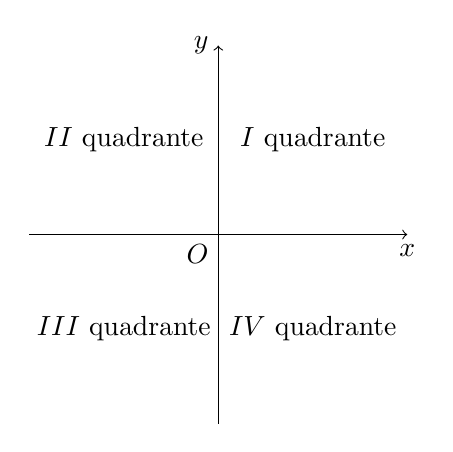
\begin{tikzpicture}[x=8mm, y=8mm, smooth]
\begin{scope}[->]
\draw (0,0) -- (6,0) node [below]  {$x$};
\draw (3,-3) -- (3,3)node [left]  {$y$};;
\end{scope}

\node[below left] at (3,0) {$O$};
\node () at (4.5,1.5) {$I$ quadrante};
\node () at (1.5,1.5) {$II$ quadrante};
\node () at (1.5,-1.5) {$III$ quadrante};
\node () at (4.5,-1.5) {$IV$ quadrante};
\end{tikzpicture}
 \caption{I quattro quadranti del piano cartesiano.}\label{fig:8.6}
 \end{minipage}\hfil
 \begin{minipage}[t]{.45\textwidth}
 \centering% (c) 2012 Dimitrios Vrettos - d.vrettos@gmail.com
\begin{tikzpicture}[x=8mm, y=8mm, smooth]
\begin{scope}[->]
\draw (0,0) -- (6,0) node [below]  {$x$};
\draw (3,-3) -- (3,3)node [left]  {$y$};;
\end{scope}

\begin{scope}[dashed, orange]
%\draw (-1,0) -- (-1,1);
%\draw (-1,1) -- (0,1);
\draw (4,0) -- (4,1.5);
\draw (4,1.5) -- (3,1.5);
\end{scope}

\filldraw[fill=CornflowerBlue, draw=black] (4,1.5)circle (1.5pt) node[above right] {$P$};
\filldraw[fill=CornflowerBlue, draw=black] (3,1.5)circle (1.5pt) node[left]{$\beta$};
\filldraw[fill=CornflowerBlue, draw=black] (4,0)circle (1.5pt) node[below] {$\alpha$};

\node[below left] at (3,0) {$O$};
\node[above] at (6,0) {$\insR^{+}$};
\node[above right] at (0,0) {$\insR^{-}$};
\node[below right] at (3,3) {$\insR^{+}$};
\node[above right] at (3,-3) {$\insR^{-}$};
\end{tikzpicture}
 \caption{Numeri positivi e negativi sul piano cartesiano.}\label{fig:8.7}
 \end{minipage}
\end{figure}

Per rappresentare gli elementi di~$\insR\times \insR$ cioè le coppie ordinate di numeri reali~$(\alpha; \beta)$ procediamo nel seguente modo:
\begin{itemize*}
\item determiniamo sull'asse~$x$ il punto~$A$ immagine del numero reale~$\alpha$;
\item da~$A$ tracciamo la retta parallela all'asse~$y$;
\item determiniamo sull'asse~$y$ il punto~$B$ immagine del numero reale~$\beta$;
\item da~$B$ tracciamo la retta parallela all'asse~$x$.
\end{itemize*}
Il punto~$P$, intersezione delle rette tracciate, è l'immagine della coppia ordinata~$(\alpha; \beta)$ (figura~\ref{fig:8.7}).  Il punto~$O$, immagine della coppia~$(0;0)$, è chiamato \emph{origine} del sistema di riferimento.

\begin{figure}[bt]
 \begin{minipage}[t]{.3\textwidth}
 \centering% (c) 2012 Dimitrios Vrettos - d.vrettos@gmail.com
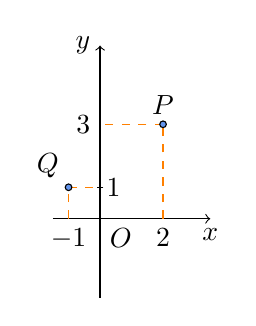
\begin{tikzpicture}[scale=.8, x=5mm, y=5mm, smooth]
\begin{scope}[->]
\draw (-1.5,0) -- (3.5,0) node [below]  {$x$};
\draw (0,-2.5) -- (0,5.5)node [left]  {$y$};;
\end{scope}

\begin{scope}[dashed, orange]
\draw (-1,0) -- (-1,1);
\draw (-1,1) -- (0,1);
\draw (2,0) -- (2,3);
\draw (2,3) -- (0,3);
\end{scope}

%\draw (1,1.5pt) -- (1,-1.5pt) node[below] {1};
\draw (1.5pt,1) -- (-1.5pt,1) node[right] {1};
\node[below right]  at (0,0){$O$};
\filldraw[fill=CornflowerBlue, draw=black] (2,3)circle (1.5pt) node[above] {$P$};
\node[left] at (0,3) {$3$};
\filldraw[fill=CornflowerBlue, draw=black] (-1,1)circle (1.5pt) node[above left] {$Q$};
\node[below] at (2,0) {$2$};
\node[below] at (-1,0) {$-1$};
\end{tikzpicture}

 \caption{}\label{fig:8.8}
 \end{minipage}\hfil
 \begin{minipage}[t]{.45\textwidth}
 \centering% (c) 2012 Dimitrios Vrettos - d.vrettos@gmail.com
\begin{tikzpicture}[scale=.8, x=5mm, y=5mm, smooth]
\begin{scope}[->]
\draw (-5.5,0) -- (4.5,0) node [below]  {$x$};
\draw (0,-2.5) -- (0,5.5)node [left]  {$y$};;
\end{scope}

\node[below] at (3,0){3};
\node[below] at (-5,0){$-5$};
\node[left] at (0,4){$4$};
\node[left] at (0,-2){$-2$};

\node[below left]  at (0,0){$O$};
\filldraw[fill=CornflowerBlue, draw=black] (3,0)circle (1.5pt) node[above] {$K$};
\filldraw[fill=CornflowerBlue, draw=black] (0,4)circle (1.5pt) node[right]{$R$};
\filldraw[fill=CornflowerBlue, draw=black] (-5,0)circle (1.5pt) node[above] {$H$};
\filldraw[fill=CornflowerBlue, draw=black] (0,-2)circle (1.5pt) node[right]{$S$};
\end{tikzpicture}
 \caption{}\label{fig:8.9}
 \end{minipage}\hfil
 \begin{minipage}[t]{.25\textwidth}
 \centering% (c) 2012 Dimitrios Vrettos - d.vrettos@gmail.com
\begin{tikzpicture}[scale=.8, x=5mm, y=5mm, smooth]
\begin{scope}[->]
\draw (-1.5,0) -- (4.5,0) node [below]  {$x$};
\draw (0,-2.5) -- (0,5.5)node [left]  {$y$};;
\end{scope}

\begin{scope}[orange,dashed]
\draw (0,4) -- (3,4)--(3,0);
\end{scope}
\node[below left]  at (0,0){$O$};
\filldraw[fill=CornflowerBlue, draw=black] (3,0)circle (1.5pt) node[below] {$\alpha$};
\filldraw[fill=CornflowerBlue, draw=black] (3,4)circle (1.5pt) node[right]{$R$};
\filldraw[fill=CornflowerBlue, draw=black] (0,4)circle (1.5pt) node[left]{$\beta$};
\end{tikzpicture}
 \caption{Ascissa e ordinata di un punto.}\label{fig:8.10}
\end{minipage}
 \end{figure}

\begin{exrig}
 \begin{esempio}
 \label{ex:8.12}
Determiniamo l'immagine delle coppie ordinate~$(2;3)$ e~$(-1;1)$.

Nella figura~\ref{fig:8.8} è tracciata la costruzione descritta sopra:~$P$ è il punto del piano immagine della coppia~$(2;3)$ e~$Q$
è il punto immagine della coppia~$(-1;1)$. Rappresenta le coppie~$(4;-1)$ e~$(-4;1)$.
Quali punti rappresentano le coppie con un elemento uguale a zero?
 \end{esempio}

 \begin{esempio}
 \label{ex:8.13}
Determiniamo l'immagine delle seguenti coppie:~$(0;4)$, $(0;-2)$, $(-5;0)$, $(3;0)$.

Osserviamo nella figura~\ref{fig:8.9} che il punto immagine dello zero sull'asse~$x$ coincide con~$O$, quindi la coppia~$(0;4)$ sarà associata al punto~$R$
dell'asse~$y$ e la coppia~$(0;-2)$ al punto~$S$ dello stesso asse. Analogamente, poiché il punto immagine dello zero sull'asse~$y$
coincide con~$O$, le coppie~$(-5;0)$ e~$(3;0)$ sono associate rispettivamente ai punti~$H$ e~$K$ dell'asse~$x$.
 \end{esempio}
\end{exrig}

\paragraph{Prima conclusione:} ogni coppia di numeri reali è rappresentata da un punto del piano dotato di riferimento cartesiano ortogonale
monometrico.

Prendiamo ora un punto~$R$ (figura~\ref{fig:8.10} a pagina~\pageref{fig:8.10}) del piano sul quale sia stato fissato un riferimento cartesiano ortogonale monometrico e tracciamo da~$R$
la parallela all'asse~$y$ che interseca l'asse~$x$ nel punto~$A$. A questo punto è associato un numero reale~$\alpha$.
Analogamente da~$R$ tracciamo la parallela all'asse~$x$ che interseca l'asse~$y$ nel punto~$B$ immagine di un numero reale~$\beta$.
Al punto~$R$ associamo la coppia di numeri reali~$(\alpha; \beta)$.

Diremo che~$R$ è il punto di coordinate~$(\alpha;\beta )$, $\alpha~$ si chiama \emph{ascissa} del punto~$R$ e $\beta$ \emph{ordinata}
del punto~$R$. Spesso le coordinate del punto $R$ sono indicate con $(x_R;y_R)$.

\paragraph{Seconda conclusione:} ogni punto del piano dotato di riferimento cartesiano ortogonale monometrico individua una coppia ordinata
di numeri reali.

In conclusione, esiste una corrispondenza biunivoca tra l'insieme~$\insR\times \insR$ e l'insieme dei punti del piano dotato di
riferimento cartesiano ortogonale monometrico. Possiamo dunque ``confondere'' coppia di numeri reali con punto del piano e
diremo, secondo gli esempi precedenti, ``$P$ è il punto~$(2;3)$'' o ``$P$
è il punto immagine della coppia~$(2;3)$'' o ancora ``$P$ è il punto di coordinate~$(2;3)$''.

\subsubsection*{Un po' di storia}
Nel~$II$~secolo~\aC\ Ipparco\footnote{noto anche come Ipparco di Nicea o di Rodi, è stato un astronomo, matematico e geografo della Grecia antica (190 \aC - 120 \aC).} compilò il primo catalogo stellare in cui precisò la posizione di circa~850 stelle sulla sfera celeste
mediante due numeri: latitudine e longitudine. La posizione di un punto era dunque individuata attraverso una coppia di numeri.
Ancora oggi attraverso latitudine e longitudine viene individuato un punto sulla superficie terrestre.
I romani, nel fondare una città, segnavano due solchi perpendicolari (cardo e decumano) ai quali riferivano la posizione di case, monumenti, strade.

Nel~$XVII$~secolo con le opere di Pierre de Fermat\footnote{matematico e magistrato francese (1601 - 1665).} e di René Descartes\footnote{filosofo e matematico francese noto anche con il nome italianizzato Renato Cartesio (1596 - 1650).} il metodo di rappresentare punti con coppie di numeri divenne
un procedimento matematico per descrivere enti geometrici attraverso numeri, equazioni, disequazioni e tradurre le relazioni
tra elementi della geometria in relazioni tra enti dell'algebra.

La geometria analitica tratta quindi questioni geometriche con metodi di tipo algebrico.

\vspazio\ovalbox{\risolvi \ref{ese:8.20}}

\subsection{Distanza tra due punti}
Assegnato nel riferimento cartesiano ortogonale il punto~$P(\alpha; \beta)$, il numero reale~$|\alpha|$ rappresenta la
misura della distanza del punto~$P$ dall'asse~$y$ e il numero reale~$|\beta|$ rappresenta la misura della distanza di~$P$
dall'asse~$x$.

\begin{figure}[b]
 \begin{minipage}[t]{.45\textwidth}
 \centering% (c) 2012 Dimitrios Vrettos - d.vrettos@gmail.com
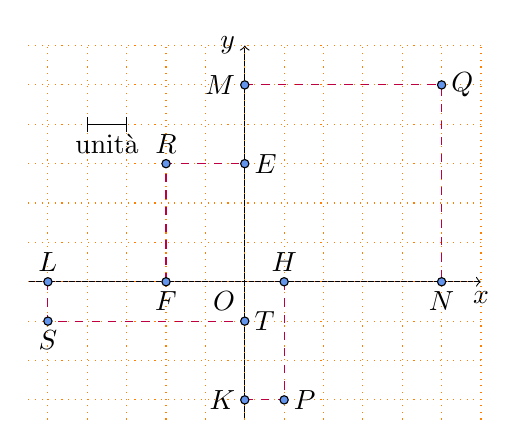
\begin{tikzpicture}[x=5mm, y=5mm, smooth]
  \begin{scope}[->]
    \draw (-5.5,0) -- (6,0) node [below]  {$x$};
    \draw (0,-3.5) -- (0,6)node [left]  {$y$};;
  \end{scope}

  \draw[orange, dotted, step=5mm] (-5.5,-3.5) grid (6,6);
  
  \begin{scope}[purple,dashed]
    \draw (-5,0) -- (-5,-1) --(0,-1);
    \draw (-2,0) -- (-2,3) --(0,3);
    \draw (1,0) -- (1,-3)--(0,-3);
    \draw (0,5) -- (5,5)--(5,0);
  \end{scope}

  \draw[|-|] (-4,4) -- (-3,4) node[below, midway] {unità};

  \node[below left]  at (0,0){$O$};
  
  \begin{scope}[fill=CornflowerBlue, draw=black]
    \filldraw (1,-3)circle (1.5pt) node[right] {$P$};
    \filldraw (5,5)circle (1.5pt) node[right]{$Q$};
    \filldraw (-2,3)circle (1.5pt) node[above] {$R$};
    \filldraw (-5,-1)circle (1.5pt) node[below]{$S$};

    \filldraw (-5,0)circle (1.5pt) node[above]{$L$};
    \filldraw (-2,0)circle (1.5pt) node[below]{$F$};
    \filldraw (0,5)circle (1.5pt) node[left]{$M$};
    \filldraw (0,3)circle (1.5pt) node[right]{$E$};
    \filldraw (0,-1)circle (1.5pt) node[right]{$T$};
    \filldraw (0,-3)circle (1.5pt) node[left]{$K$};
    \filldraw (1,0)circle (1.5pt) node[above]{$H$};
    \filldraw (5,0)circle (1.5pt) node[below]{$N$};
  \end{scope}
\end{tikzpicture}
 \caption{}\label{fig:8.11}
 \end{minipage}\hfil
 \begin{minipage}[t]{.45\textwidth}
 \centering% (c) 2012 Dimitrios Vrettos - d.vrettos@gmail.com
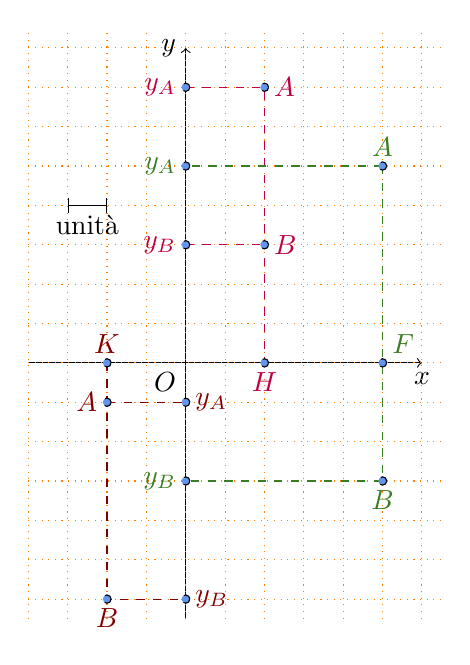
\begin{tikzpicture}[x=5mm, y=5mm, smooth]
  \begin{scope}[->]
    \draw (-4,0) -- (6,0) node [below]  {$x$};
    \draw (0,-6.5) -- (0,8)node [left]  {$y$};;
  \end{scope}

  \draw[dotted,orange, step=5mm] (-4,-6.5) grid (6.5,8.5);

  \draw[|-|] (-3,4) -- (-2,4) node[below, midway] {unità};

  \node[below left]  at (0,0){$O$};
  
  \begin{scope}[every node/.style={purple}, draw=purple, dashed]
    \draw (0,7) -- (2,7)--(2,0);
    \draw (0,3) -- (2,3);
    \begin{scope}[fill=CornflowerBlue, draw=black]
      \filldraw (2,3)circle (1.5pt) node[right, purple] {$B$};
      \filldraw (2,7)circle (1.5pt) node[right]{$A$};
      \filldraw (0,7)circle (1.5pt) node[left]{$y_A$};
      \filldraw (0,3)circle (1.5pt) node[left]{$y_B$};
      \filldraw (2,0)circle (1.5pt) node[below]{$H$};
    \end{scope}
  \end{scope}

  \begin{scope}[every node/.style={OliveGreen},draw=OliveGreen,dashed]
    \draw (5,5) -- (5,-3)--(0,-3);
    \draw (5,5) -- (0,5);
    \begin{scope}[fill=CornflowerBlue, draw=black]
      \filldraw (5,5)circle (1.5pt) node[above] {$A$};
      \filldraw (0,5)circle (1.5pt) node[left]{$y_A$};

      \filldraw (5,-3)circle (1.5pt) node[below]{$B$};
      \filldraw (0,-3)circle (1.5pt) node[left]{$y_B$};

      \filldraw (5,0)circle (1.5pt) node[above right]{$F$};
    \end{scope}
  \end{scope}

  \begin{scope}[every node/.style={Maroon}, draw=Maroon, dashed]
    \draw (-2,0) -- (-2,-6) --(0,-6);
    \draw (-2,-1) -- (0,-1);
    \begin{scope}[fill=CornflowerBlue, draw=black]
      \filldraw (-2,-1)circle (1.5pt) node[left] {$A$};
      \filldraw (0,-1)circle (1.5pt) node[right]{$y_A$};

      \filldraw (-2,-6)circle (1.5pt) node[below]{$B$};
      \filldraw (0,-6)circle (1.5pt) node[right]{$y_B$};

      \filldraw (-2,0)circle (1.5pt) node[above]{$K$};
    \end{scope}
  \end{scope}
\end{tikzpicture}
 \caption{}\label{fig:8.12}
 \end{minipage}
 \end{figure}
\pagebreak
\begin{exrig}
 \begin{esempio}
 \label{ex:8.14}
Determinare la misura della distanza dagli assi coordinati dei punti~$P(+1;-3)$, $Q(+5;+5)$, $R(-2;+3)$, $S(-5;-1)$ (figura~\ref{fig:8.11}).

\emph{Dati}:~$P(+1;-3)$.

\emph{Obiettivo}:~$PH\perp$ asse~$x$, il segmento~$PH$ è la distanza di~$P$ dall'asse~$x$;
$PK\perp$ asse~$y$, il segmento~$PK$ è la distanza di~$P$ dall'asse~$y$.

Per quanto detto sopra si ha~$\overline{PH}=|-3|=-(-3)=3$; $\overline{PH}=|+1|=1$.
Completate la soluzione dell'esempio, seguendo la traccia.
 \end{esempio}
\end{exrig}

Vogliamo ora determinare la misura~$\overline{AB}$ di un segmento~$AB$, inserito in un riferimento cartesiano ortogonale
monometrico~$O_{xy}$, conoscendo le coordinate degli estremi~$A$ e~$B$ del segmento stesso.

\begin{figure}[t]
 \begin{minipage}[t]{.45\textwidth}
 \centering% (c) 2012 Dimitrios Vrettos - d.vrettos@gmail.com
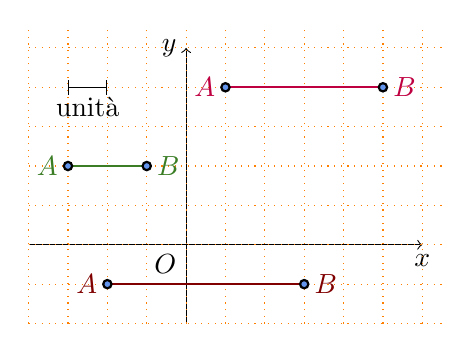
\begin{tikzpicture}[x=5mm, y=5mm, smooth]
  \begin{scope}[->]
    \draw (-4,0) -- (6,0) node [below]  {$x$};
    \draw (0,-2) -- (0,5)node [left]  {$y$};;
  \end{scope}

  \draw[dotted,orange, step=5mm] (-4,-2) grid (6.5,5.5);

  \draw[|-|] (-3,4) -- (-2,4) node[below, midway] {unità};

  \node[below left]  at (0,0){$O$};
  
  \begin{scope}[every node/.style={purple}, draw=purple,thick]
    \draw (1,4) -- (5,4);
    \begin{scope}[fill=CornflowerBlue, draw=black]
      \filldraw (5,4)circle (1.5pt) node[right, purple] {$B$};
      \filldraw (1,4)circle (1.5pt) node[left]{$A$};
    \end{scope}
  \end{scope}

  \begin{scope}[every node/.style={OliveGreen},draw=OliveGreen,thick]
    \draw (-3,2) -- (-1,2);
    \begin{scope}[fill=CornflowerBlue, draw=black]
      \filldraw (-3,2)circle (1.5pt) node[left] {$A$};
      \filldraw (-1,2)circle (1.5pt) node[right]{$B$};
    \end{scope}
  \end{scope}

  \begin{scope}[every node/.style={Maroon}, draw=Maroon, thick]
    \draw (-2,-1) -- (3,-1);
    \begin{scope}[fill=CornflowerBlue, draw=black]
      \filldraw (-2,-1)circle (1.5pt) node[left] {$A$};
      \filldraw (3,-1)circle (1.5pt) node[right]{$B$};
    \end{scope}
  \end{scope}
\end{tikzpicture}
 \caption{I due punti hanno la stessa ordinata.}\label{fig:8.13}
 \end{minipage}\hfil
 \begin{minipage}[t]{.45\textwidth}
 \centering% (c) 2012 Dimitrios Vrettos - d.vrettos@gmail.com
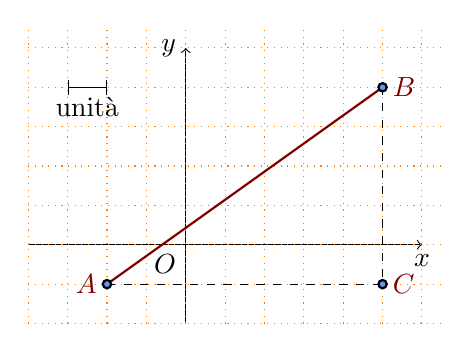
\begin{tikzpicture}[x=5mm, y=5mm, smooth]
  \begin{scope}[->]
    \draw (-4,0) -- (6,0) node [below]  {$x$};
    \draw (0,-2) -- (0,5)node [left]  {$y$};;
  \end{scope}

  \draw[dotted,orange, step=5mm] (-4,-2) grid (6.5,5.5);

  \draw[|-|] (-3,4) -- (-2,4) node[below, midway] {unità};

  \node[below left]  at (0,0){$O$};
  	\draw[dashed,thin] (-2,-1) -- (5,-1)--(5,4);
  \begin{scope}[every node/.style={Maroon}, draw=Maroon, thick]
    \draw (-2,-1) -- (5,4);
    \begin{scope}[fill=CornflowerBlue, draw=black]
      \filldraw (-2,-1)circle (1.5pt) node[left] {$A$};
      \filldraw (5,4)circle (1.5pt) node[right]{$B$};
      \filldraw (5,-1)circle (1.5pt) node[right]{$C$};

    \end{scope}
  \end{scope}
\end{tikzpicture}
 \caption{Il segmento ha una direzione diversa da quella degli assi coordinati.}\label{fig:8.14}
 \end{minipage}
 \end{figure}

\paragraph{Caso I} i due punti hanno la stessa ascissa. Il segmento~$AB$ è parallelo all'asse~$y$ e può
presentarsi in diverse posizioni rispetto all'asse~$x$ (figura~\ref{fig:8.12}).

\begin{exrig}
 \begin{esempio}
Determinare la misura della distanza tra i punti~$A(2;7)$ e~$B(2;3)$.

\emph{Dati}:~$A(2;7)$, $B(2;3)$.

\emph{Obiettivo}:~$\overline{AB}$.

\emph{Procedura risolutiva}:~$\overline{AB}=\overline{AH}-\overline{BH}=y_{A}-y_{B}=7-3=4$.

 \end{esempio}
 \begin{esempio}
 \label{ex:8.16}
Determinare la misura della distanza tra i punti~$A(5;5)$ e~$B(5;-3)$.

\emph{Dati}:~$A(5;5)$, $B(5;-3)$.

\emph{Obiettivo}:~$\overline{AB}$.

\emph{Procedura risolutiva}:~$\overline{AB}=\overline{AF}+\overline{BF}=y_{A}+(-y_{B})=y_{A}-y_{B}=5-(-3)=8$.

 \end{esempio}
 \begin{esempio}
Determinare la misura della distanza tra i punti~$A(-2;-1)$ e~$B(-2;-6)$.

\emph{Dati}:~$A(-2;-1)$, $B(-2;-6)$.

\emph{Obiettivo}:~$\overline{AB}$.

\emph{Procedura risolutiva}:~$\overline{AB}=\overline{BK}-\overline{AK}=-(y_{B})-(-y_{A})=y_{A}-y_{B}=-1+6=5$.

 \end{esempio}
\end{exrig}
Osserviamo che in ogni caso abbiamo sottratto dall'ordinata maggiore l'ordinata minore; generalizzando possiamo concludere:
la misura del segmento $AB$ parallelo all'asse delle ordinate è~$\overline{AB}=|y_{A}-y_{B}|$
indipendentemente da quale estremo abbia ordinata maggiore.

\paragraph{Caso II} i due punti hanno la stessa ordinata. Il segmento~$AB$ (figura~\ref{fig:8.13}) è parallelo all'asse~$x$ e
può presentarsi in diverse posizioni rispetto all'asse~$y$.

Seguendo il procedimento applicato nel primo caso, dopo aver rilevato le coordinate degli estremi del segmento~$AB$
nella figura~\ref{fig:8.13}, verifica che in ogni caso~$\overline{AB}=|x_{A}-x_{B}|$.

La misura del segmento $AB$ parallelo all'asse delle ascisse è~$\overline{AB}=|x_{A}-x_{B}|$
indipendentemente da quale estremo abbia ascissa maggiore.

\paragraph{Caso III} è questo il caso generale: il segmento ha una direzione diversa da quella degli assi coordinati (figura~\ref{fig:8.14}).

\emph{Dati}:~$A(x_A;x_B)$, $B(y_A;y_B)$.

\emph{Obiettivo}:~$\overline{AB}$.

\emph{Procedura risolutiva}: tracciando da~$A$ la parallela all'asse~$x$ e da~$B$ la parallela all'asse~$y$
si determina il vertice~$C$ del triangolo rettangolo~$ABC$ di cui~$AB$ è l'ipotenusa.
Per il teorema di Pitagora si ottiene:~$\overline{AB}=\sqrt{\overline{AC}^2 + \overline{BC}^2}=\sqrt{\left(x_A-x_C \right)^2+
\left(y_C-y_B \right)^2}$. %----figura18
Poiché $x_{C}=x_{B}$ e~$y_{C}=y_{A}$ sostituendo si ha:
$\overline{AB}=\sqrt{\left(x_{A}-x_{B}\right)^{2}+\left(y_{A}-y_{B}\right)^{2}}$.

La misura del segmento $AB$, note le coordinate dei suoi estremi, è quindi:
\[\overline{AB}=\sqrt{\left(x_{A}-x_{B}\right)^{2}+\left(y_{A}-y_{B}\right)^{2}}.\]

\ovalbox{\risolvii  \ref{ese:8.21}, \ref{ese:8.22}, \ref{ese:8.23}, \ref{ese:8.24}, \ref{ese:8.25}, \ref{ese:8.26},
\ref{ese:8.27}, \ref{ese:8.28}, \ref{ese:8.29}, \ref{ese:8.30}, \ref{ese:8.31}, \ref{ese:8.32}, \ref{ese:8.33}}
\pagebreak
%\vspazio\ovalbox{\ref{ese:8.31}}
\subsection{Punto medio di un segmento}
Ricordiamo il teorema di Talete:

\begin{teorema}[di Talete]
Un fascio di rette parallele tagliato da due trasversali $r$ e $r'$ determina su esse segmenti che mantengono tra loro le proporzioni, cioè $\overline{AB}:\overline{A'B'}=\overline{BC}:\overline{B'C'}$.
\end{teorema}

\begin{figure}[h]
 \centering% (c) 2012 Dimitrios Vrettos - d.vrettos@gmail.com
\begin{tikzpicture}[x=10mm, y=10mm, smooth]
\tkzSetUpPoint[shape=circle,size=7pt,color=black, fill=CornflowerBlue]
\tkzDefPoints{0/0/a1, 4/0/a2, 0/-0.8/b1, 4/-0.8/b2, 0/-2/c1, 4/-2/c2}

\tkzSetUpLine[color=Maroon]
\tkzDrawLine[end= $a$](a1,a2)
\tkzDrawLine[end= $b$](b1,b2)
\tkzDrawLine[end= $c$](c1,c2) 

%\tkzDefPoints{1/0/A, 2.8/0/A', 0/-2/C, 4/-2/C'}
\tkzDefPoints{1/0/A, 2.5/0/A', 0/-2/C, 4/-2/C'}

\tkzDefLine(C,A)
\tkzInterLL(C,A)(b1,b2) \tkzGetPoint{B}

\tkzDefLine(C',A')
\tkzInterLL(C',A')(b1,b2) \tkzGetPoint{B'}

\tkzSetUpLine[color=OliveGreen]
\tkzDrawLine[end= $r$](C,A)
\tkzDrawLine[end= $r'$](C',A')

\tkzDrawPoints(A,A',B,B',C,C')
\tkzLabelPoints[above left](A,B,C)
\tkzLabelPoints[above right](A',B',C')
\end{tikzpicture}
 \caption{Il teorema di Talete.}\label{fig:8.15}
 \end{figure}

Richiamiamo anche la definizione di punto medio di un segmento:
\begin{definizione}
 Il \emph{punto medio di un segmento}~$AB$ è il punto $M$ interno
al segmento che lo divide in due parti congruenti:~$\overline{AM}=\overline{MB}$.
\end{definizione}

  \begin{figure}[h]
  \centering% (c) 2012 Dimitrios Vrettos - d.vrettos@gmail.com
\begin{tikzpicture}[x=10mm, y=10mm, smooth]
	\tkzSetUpPoint[shape=circle,size=7pt,color=black, fill=CornflowerBlue]

	\tkzDefPoint(0,2){A}
	\tkzDefPoint(4,2){B}
	\tkzDefMidPoint(A,B) 
	\tkzGetPoint{M}
	
	\tkzDrawSegment[style={thick, Maroon}](A,B)    
	\tkzLabelPoints[above](A,B,M)

	\tkzDrawPoints(A,B,M)

\end{tikzpicture}
  \caption{Il punto medio.}\label{fig:8.16}
 \end{figure}

%\pagebreak
%\begin{problema}
%\begin{exrig}
% \begin{esempio}
%\label{ex:8.18}
Se si conoscono le coordinate degli estremi~$A(x_A;y_a)$ e~$B(x_B;y_B)$ di un segmento possiamo determinare
le coordinate del suo punto medio $M(x_{M};y_{M})$ (figura~\ref{fig:8.17}).
\begin{figure}[hbt]
   \centering% (c) 2012 Dimitrios Vrettos - d.vrettos@gmail.com
\begin{tikzpicture}[x=10mm, y=10mm, smooth, scale=.8]
  \tikzset{xaxe style/.style ={->}}

  \tkzInit[xmin=-.5,xmax=5,ymin=-.5,ymax=4]

  \clip (-1,-.5) rectangle (6,5);

  \tkzDrawX[noticks,below]
  \tkzDrawY[noticks] 

  \tkzSetUpPoint[shape=circle,size=7pt,color=black, fill=CornflowerBlue]

  \tkzDefPoint(0,0){o}
  \tkzDefPoint(6,0){x}
  \tkzDefPoint(0,5){y}

  \tkzDefPoint(0,0){O}
  \tkzDefPoint(1,4){A}
  \tkzDefPoint(5,2){B}
  \tkzDefMidPoint(A,B) 
  \tkzGetPoint{M}

  \tkzDrawSegment[style={thick, Maroon}](A,B)    
  \tkzLabelPoints[above](A,B,M)

  \tkzDefPointBy[projection=onto o--x](A) \tkzGetPoint{A'}
  \tkzDefPointBy[projection=onto o--x](B) \tkzGetPoint{B'}
  \tkzDefPointBy[projection=onto o--x](M) \tkzGetPoint{M'}

  \tkzDefPointBy[projection=onto o--y](A) \tkzGetPoint{A''}
  \tkzDefPointBy[projection=onto o--y](B) \tkzGetPoint{B''}
  \tkzDefPointBy[projection=onto o--y](M) \tkzGetPoint{M''}

  \tkzLabelPoints[below](A',B',M')
  \tkzLabelPoints[left](A'',B'',M'')
  \tkzLabelPoints[below left](O)

  \tkzDrawSegment[style=dashed](A,A')
  \tkzDrawSegment[style=dashed](B,B')
  \tkzDrawSegment[style=dashed](A,A'')
  \tkzDrawSegment[style=dashed](B,B'')

  \tkzDrawSegment[style=dotted](M,M')
  \tkzDrawSegment[style=dotted](M,M'')

  \tkzDrawPoints(A,B,M)
  \tkzDrawPoints(A',B',M')
  \tkzDrawPoints(A'',B'',M'')
\end{tikzpicture}
  \caption{Le coordinate del punto medio.}\label{fig:8.17}
\end{figure}

Essendo~$\overline{AM}=\overline{MB}$ per il teorema di Talete~$\overline{A'M'}=\overline{M'B'}$;
si ha inoltre~$A'(x_{A};0)$, $B'(x_{B};0)$, $M'(x_{M};0)$ e quindi~$x_{M}-x_{A}=x_{B}-x_{M}$
da cui~$2x_{M}=x_{A}+x_{B}$ e dunque~$x_{M}=\dfrac{x_{A}+x_{B}}{2}$.

Con ragionamento analogo, tracciando dai punti~$A$, $B$, $M$ le parallele all'asse~$x$, si ricava~$y_{M}=\dfrac{y_{A}+y_{B}}{2}$.

Le coordinate del punto medio $M$ di un segmento~$AB$, con~$A(x_{A};x_{B})$ e $B(x_{B};y_{B})$ sono quindi:
\[x_{M}=\dfrac{x_{A}+x_{B}}{2};\quad y_{M}=\dfrac{y_{A}+y_{B}}{2}.\]
%\end{problema}

%\begin{soluzione}
%\emph{Dati}:~$A(x_A;y_a)$, $B(x_B;y_B)$, $\overline{AM} = \overline{MB}$.

%\emph{Obiettivo}:~$M(x_{M};y_{M})$.
%
%\emph{Procedura risolutiva}: essendo~$\overline{AM}=\overline{MB}$ per il teorema di Talete~$\overline{A'M'}=\overline{M'B'}$;
%si ha inoltre~$A'(x_{A};0)$, $B'(x_{B};0)$, $M'(x_{M};0)$ e quindi~$x_{M}-x_{A}=x_{B}-x_{M}$
%da cui~$2x_{M}=x_{A}+x_{B}$ e dunque~$x_{M}=\dfrac{x_{A}+x_{B}}{2}$.
%
%Con ragionamento analogo, tracciando dai punti~$A$, $B$, $M$ le parallele all'asse~$x$, si ricava~$y_{M}=\dfrac{y_{A}+y_{B}}{2}$.
%
%Le coordinate del punto medio $M$ di un segmento~$AB$, con~$A(x_{A};x_{B})$ e $B(x_{B};y_{B})$ sono quindi:
%\[x_{M}=\dfrac{x_{A}+x_{B}}{2};\quad y_{M}=\dfrac{y_{A}+y_{B}}{2}.\]
%\end{soluzione}
%\end{esempio}

\begin{exrig}
 \begin{esempio}
Dato il segmento di estremi~$A\left(-{\frac{3}{4}};1\right)$, $B\left(2;-\frac{1}{2}\right)$ determinare le coordinate del suo punto medio $M$.

\emph{Dati}:~$A\left(-{\frac{3}{4}};1\right)$, $B\left(2;-\frac{1}{2}\right)$, $\overline{AM}=\overline{MB}$.

\emph{Obiettivo}:~$M(x_{M};y_{M})$.

\emph{Procedura risolutiva}:~$x_{M}=\frac{x_{A}+x_{B}}{2}=\frac{-{\frac{3}{4}}+2}{2}=\frac{5}{8}$;\,
$y_{M}=\frac{1+\left(-{\frac{1}{2}}\right)}{2}=\frac{1}{4}$ quindi~$M\left(\frac{5}{8};\frac{1}{4}\right)$.
 \end{esempio}
\end{exrig}

\ovalbox{\risolvii \ref{ese:8.34}, \ref{ese:8.35}, \ref{ese:8.36}, \ref{ese:8.37}, \ref{ese:8.38}}

%\pagebreak

\section{Il grafico di una funzione}

Ricordiamo le definizioni \ref{def:funzione} e \ref{def:immagine_di_f}. Una funzione~$f$ è una corrispondenza univoca tra due insiemi non vuoti: ad ogni elemento~$x$ (variabile indipendente) del dominio associa uno e un solo valore~$y$ del codominio (variabile dipendente).
L'elemento~$y$, corrispondente di un elemento~$x$ del dominio, viene detto immagine di~$x$ nella funzione~$f$ e si scrive~$y=f(x)$.

Le funzioni numeriche, cioè aventi per dominio e codominio insiemi numerici, possono essere espresse:
\begin{itemize}
\item con \emph{linguaggio comune}, purché in modo preciso e inequivocabile (esempio: La funzione~$f$
 ``associa ad ogni numero razionale il suo triplo'');
\item attraverso un \emph{algoritmo} (figura~\ref{fig:8.18}), cioè una serie di istruzioni per trasformare il valore della variabile indipendente
 (in ingresso) nel valore della variabile dipendente (in uscita);
\begin{figure}[hb]
\centering% (c) 2012 Dimitrios Vrettos - d.vrettos@gmail.com
\begin{tikzpicture} [scale=.8,auto,block/.style={rectangle, draw=Maroon, thick, text width=5.3em,align=center, rounded corners, minimum height=4em},%
block1/.style={rectangle, draw=Maroon, thick, text width=8em,align=center, rounded corners, minimum height=4em},%
cloud/.style={draw=CornflowerBlue, thick, ellipse, minimum height=2.2em},%
line/.style ={draw, thick, ->,shorten >=2pt}]

  \matrix [column sep=7mm]{
    \node [block] (prn) {prendi un numero razionale}; 
    & \node [block] (molt) {moltiplicalo per 3}; 
    & \node [block] (scr) {scrivi il risultato}; \\
  };
  
  \begin{scope}[every path/.style=line]
    \path (prn)-- (molt);
    \path (molt) -- (scr);
  \end{scope}

  \begin{scope}[yshift=-30mm]
    \matrix [column sep=14mm, row sep=7mm]{
      \node [block1] (ind) {Variabile indipendente: $x$}; 
      & \node [block1] (dip) {Variabile dipendente: $y$}; \\
      \node[cloud] (ing) {Valore in ingresso};
      &\node[cloud] (usc) {Valore in uscita};\\
    };

    \begin{scope}[every path/.style=line]
      \path (ind)--  node [midway]{$f$} (dip);
      \path (ing) --(ind);
      \path(dip)--(usc);
    \end{scope}
  \end{scope}
\end{tikzpicture}
  
\caption{Funzione numerica espressa tramite un algoritmo.}\label{fig:8.18}
\end{figure}
\pagebreak
\item mediante una \emph{tabella}:
 \begin{center}
\begin{tabular}{cccccc}
 \toprule
 $x$ & $-2$ & $0$ & $3$ & $7$ & $10$ \\
 $y$ & $-6$ & $0$ & $9$ & $21$ & $30$\\
 \bottomrule
 \end{tabular}
 \end{center}
\item con una \emph{formula} che indica il calcolo che si effettua sulla variabile indipendente per determinare in modo univoco
il valore della variabile dipendente. Per esempio:~$y=3x$.
\end{itemize}

\begin{exrig}
 \begin{esempio}
Traccia su un piano quadrettato un riferimento cartesiano ortogonale monometrico.
Completa la tabella per la funzione~$y=2x$ avente come dominio e codominio l'insieme~$\insR$ dei numeri reali.
\begin{center}
 \begin{tabular}{ccccccc}
 \toprule
 $x$ & $0$ && $1/2$ & $2$ & $-3$ &\\
 $y$ &&$2$&&&&$5$\\
 \bottomrule
 \end{tabular}
\end{center}
Ogni coppia~$(x;y)$ determina nel riferimento cartesiano un punto; rappresenta i punti le cui coordinate sono
le coppie ordinate contenute nella tabella. Puoi osservare che i punti trovati sono allineati su una retta passante
per l'origine del riferimento.
 \end{esempio}
\end{exrig}
\begin{definizione}
 Si chiama \emph{grafico di una funzione} l'insieme di tutti e soli i punti del piano cartesiano che
 rappresentano le coppie ordinate costruite tramite la funzione assegnata.
\end{definizione}
\osservazione
I pochi punti ottenuti dalla compilazione della tabella possono essere uniti con un tratto continuo perché
assegnando alla variabile indipendente altri valori reali, ad esempio compresi tra~$0$ e~$2$, si potrebbero
determinare infiniti punti che risulterebbero allineati con i precedenti.

\vspazio\ovalbox{\risolvii \ref{ese:8.39}, \ref{ese:8.40}}

\subsection{Funzione di proporzionalità diretta}
\begin{center}
 \begin{tabular}{ccccccc}
 \toprule
 $x$ & $0$ & $-1$ & $ 1/2$ & $2$ & $-3$ & $-5/2$\\
 $y$ & $0$ & $2$ & $-1$ & $-4$ & $6$ & $5$\\
 \midrule
 $y/x$ & & & & & & \\
 \bottomrule
 \end{tabular}
\end{center}
Compila la terza riga della tabella contenente il rapporto tra la variabile dipendente~$y$ e la variabile indipendente~$x$.
Cosa osservi? Completa:~$\dfrac{y}{x}=\dotfill$
\begin{definizione}
 Una funzione in cui risulta costante e diverso da zero il rapporto tra la variabile dipendente e la variabile indipendente
 si chiama \emph{funzione di proporzionalità diretta}. In simboli, $y$ direttamente proporzionale a
$x \Leftrightarrow \dfrac{y}{x}=k$ con~$k\in \insR$ e~$k\neq~0$ o anche~$y=k\cdot x$.
\end{definizione}
Il grafico di una funzione di proporzionalità diretta è una \emph{retta passante per l'origine};
la costante~$k$ si chiama \emph{coefficiente angolare} della retta.

Nella figura~\ref{fig:8.19} è rappresentata una retta passante per l'origine del riferimento; essa forma con l'asse orientato delle
$x$ un angolo~$\alpha~$; la costante~$k$ ci dà informazioni su tale angolo.
In particolare se la costante di proporzionalità è \emph{positiva}, l'angolo~$\alpha$ è \emph{acuto}, se la costante è
\emph{negativa} allora l'angolo~$\alpha$ è \emph{ottuso}. Se $k=1$ l'angolo è di~45° e la retta è la bisettrice del I e III quadrante.

\begin{figure}[hb]
 \begin{minipage}[t]{.45\textwidth}
  \centering% (c) 2012 Dimitrios Vrettos - d.vrettos@gmail.com
\begin{tikzpicture}[x=10mm, y=10mm, smooth,scale=.9]
  \tikzset{xaxe style/.style ={->}}
  \tkzInit[xmin=-.5,xmax=3,ymin=-.5,ymax=3]

  \clip (-.5,-.5) rectangle (4,4);

  \tkzDefPoint(0,0){o}
  \tkzDefPoint(6,0){x}

  \tkzDefPoint(0,0){O}
  \tkzDefPoint(1,0){A}
  \tkzDefPoint(2,2){B}

  \tkzMarkAngle[arc=l,size=1 cm,fill=LimeGreen](A,O,B)
  \tkzLabelAngle[pos=1.3](A,O,B){$\alpha$}

  \tkzDrawX[noticks,below]
  \tkzDrawY[noticks] 

  \tkzLabelPoints[above left](O)

  \draw[Maroon, thick] (-.5,-.5)--(3,3);
\end{tikzpicture}
  \caption{Coefficiente angolare di una funzione.}\label{fig:8.19}
 \end{minipage}\hfil
 \begin{minipage}[t]{.45\textwidth}
  \centering% (c) 2012 Dimitrios Vrettos - d.vrettos@gmail.com
\begin{tikzpicture}[x=10mm, y=10mm,scale=.9]

\clip (-.5,-.5) rectangle (4,4);

\tkzDefPoint(0,0){A}
\tkzDefPoint(3,0){B}
\tkzDefPoint(3,3){C}
\tkzDefPoint(0,3){D}

\tkzDrawSegment(A,B)
\tkzDrawSegment(C,B)
\tkzDrawSegment(C,D)
\tkzDrawSegment(A,D)

 \tkzLabelPoints[below left](A)
 \tkzLabelPoints[below right](B)
 \tkzLabelPoints[above right](C)
 \tkzLabelPoints[above left](D)

\draw[CornflowerBlue, thick] (0,0)--(3,3);
\end{tikzpicture}
  \caption{}\label{fig:8.20}
 \end{minipage}
\end{figure}


\begin{problema}
\label{ex:8.21}
Nel quadrato~$ABCD$ di figura~\ref{fig:8.20} il cui lato misura~$x$, determinare il perimetro e la diagonale.
\end{problema}
\begin{soluzione}
 Abbiamo i dati:~$\overline{AB}=x$ con~$x>0$ e l'obiettivo:~$2p$, $\overline{AC}$.

 $2p=4\cdot x$, al variare del lato varia il perimetro, che risulta essere dunque funzione del lato.
Indicato con~$y$ il perimetro scriviamo~$y=4x$, funzione di proporzionalità diretta con~$\Dom=\insR^{+}$,
coefficiente~$k=4$. La rappresentazione grafica di questa funzione è una semiretta contenuta nel primo quadrante,
ma privata del suo punto origine (figura~\ref{fig:8.21}).

Determiniamo ora la diagonale: per il teorema di Pitagora si ha
\begin{align*}
 &\overline{AC}^{2}=\overline{AB}^{2}+\overline{BC}^{2}=x^{2}+x^{2}=2x^{2}\\
 \Rightarrow\:&\overline{AC}=\sqrt{2\cdot x^{2}}=x\cdot \sqrt{2}.
\end{align*}

\begin{figure}[htb]
 \begin{minipage}[b]{.45\textwidth}
  \centering% (c) 2012 Dimitrios Vrettos - d.vrettos@gmail.com
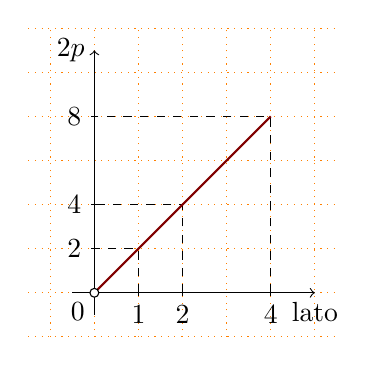
\begin{tikzpicture}[x=7mm, y=7mm, smooth,scale=.8]
\begin{scope}[dotted,orange]
\draw[step=7mm] (-1.5,-1) grid (5.5,6);
\end{scope}
\begin{scope}[->]
\draw (-.5,0) -- (5,0) node [below]  {lato};
\draw (0,-.5) -- (0,5.5) node [left]   {$2p$};
\end{scope}
\foreach \x/\xtext in {1/1,2/2,4/4}
\draw (\x,1.5pt) -- (\x,-1.5pt) node[below] {\xtext};
\foreach \y/\ytext in {1/2,2/4,4/8}
\draw (1.5pt,\y) -- (-1.5pt,\y) node[left] {$\ytext$};

\begin{scope}[dashed]
\draw (1,0) -- (1,1) --(0,1);
\draw (2,0) -- (2,2) --(0,2);
\draw (4,0) -- (4,4) --(0,4);
\end{scope}
\draw[Maroon, thick] (0,0)--(4,4);


\node[below left] at (0,0) {0};
\filldraw[fill=white, draw=black] (0,0) circle (2pt);

\end{tikzpicture}
  \caption{Il perimetro~$2p$ in funzione del lato.}\label{fig:8.21}
 \end{minipage}\hfil
 \begin{minipage}[b]{.45\textwidth}
  \centering% (c) 2012 Dimitrios Vrettos - d.vrettos@gmail.com
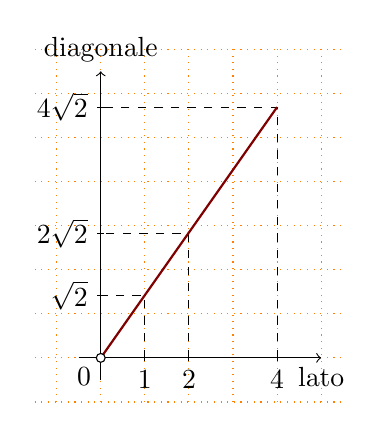
\begin{tikzpicture}[x=7mm, y=7mm, smooth,scale=.8]
\begin{scope}[dotted,orange]
\draw[step=7mm] (-1.5,-1) grid (5.5,7);
\end{scope}
\begin{scope}[->]
\draw (-.5,0) -- (5,0) node [below]  {lato};
\draw (0,-.5) -- (0,6.5) node [above]   {diagonale};
\end{scope}
\foreach \x/\xtext in {1/1,2/2,4/4}
\draw (\x,1.5pt) -- (\x,-1.5pt) node[below] {\xtext};
\foreach \y/\ytext in {1.414/\sqrt{2},2.828/2\sqrt{2},5.687/4\sqrt{2}}
\draw (1.5pt,\y) -- (-1.5pt,\y) node[left] {$\ytext$};

\begin{scope}[dashed]
\draw (1,0) -- (1,1.414) --(0,1.414);
\draw (2,0) -- (2,2.828) --(0,2.828);
\draw (4,0) -- (4,5.687) --(0,5.687);
\end{scope}
\draw[Maroon, thick] (0,0)--(4,5.687);


\node[below left] at (0,0) {0};
\filldraw[fill=white, draw=black] (0,0) circle (2pt);

\end{tikzpicture}
  \caption{La diagonale in funzione del lato.}\label{fig:8.22}
 \end{minipage}
\end{figure}

Indicando con~$y$ la diagonale si ha la funzione di proporzionalità diretta~$y=\sqrt{2}\cdot x$
con coefficiente~$k=\sqrt{2}$, di dominio~$\Dom=\insR^{+}$.
La rappresentazione grafica di questa funzione è una semiretta contenuta nel primo quadrante, ma privata del suo punto origine (figura~\ref{fig:8.22}).
\end{soluzione}

\vspazio\ovalbox{\risolvii \ref{ese:8.41}, \ref{ese:8.42}, \ref{ese:8.43}, \ref{ese:8.44}, \ref{ese:8.45}}
\pagebreak
\subsection{La funzione costante}

La figura~\ref{fig:8.23} rappresenta una funzione in cui~$\Dom=\insR$ e l'insieme~$\IM=\{2\}$.

\begin{figure}[h]
 \begin{minipage}[b]{.50\textwidth}
  \centering% (c) 2012 Dimitrios Vrettos - d.vrettos@gmail.com
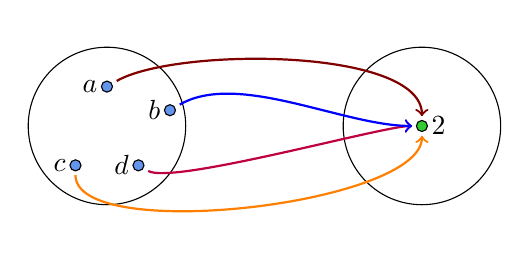
\begin{tikzpicture}[x=10mm, y=10mm]
    \node[circle, minimum height=2cm,draw] (A) at (0,0) {};
    \node[above] (A1) at (A.north) {$\Dom$};

    \begin{scope}[fill=CornflowerBlue]
      \filldraw (0,.5) circle (2pt) node (a) {};
      \node[left] at (0,.5) {$a$};
      \filldraw (.8,.2) circle (2pt) node (b) {};
      \node[left] at (.8,.2) {$b$};
      \filldraw (-.4,-.5) circle (2pt) node (c) {};
      \node[left] at (-.4,-.5)  {$c$};
      \filldraw (.4,-.5) circle (2pt) node (d) {};
      \node[left] at (.4,-.5)  {$d$};
    \end{scope}
    
    
    \begin{scope}[xshift=4cm]
    \node[circle, minimum height=2cm,draw] (B) at (0,0) {};
    \node[above] (B1) at (B.north) {$\IM$};

      \begin{scope}[fill=LimeGreen]
	\filldraw (0,0) circle (2pt)node (b1) {};
	\node[right] at (0,0) {$2$};
      \end{scope}
    \end{scope}

    \begin{scope}[->,smooth,thick]
      \draw[Maroon] (a) .. controls +(30:1cm) and +(90:1cm) .. (b1);
      \draw[purple] (d) .. controls +(-30:.5cm) and +(180:0.5cm) .. (b1);
      \draw[orange] (c) .. controls +(-90:1cm) and +(-90:1cm) .. (b1);
    \draw[blue] (b) .. controls +(30:1cm) and +(180:1cm) .. (b1);
         
 \end{scope}

\end{tikzpicture}
  \caption{Funzione con~$\Dom=\insR$ e~$\IM=\{2\}$.}\label{fig:8.23}
 \end{minipage}\hfil
 \begin{minipage}[b]{.4\textwidth}
  \centering% (c) 2012 Dimitrios Vrettos - d.vrettos@gmail.com
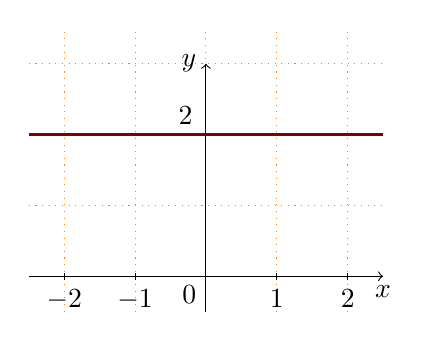
\begin{tikzpicture}[x=10mm, y=10mm, smooth,scale=.9]
\begin{scope}[dotted,orange]
\draw[step=10mm] (-2.5,-.5) grid (2.5,3.5);
\end{scope}
\begin{scope}[->]
\draw (-2.5,0) -- (2.5,0) node [below]  {$x$};
\draw (0,-.5) -- (0,3) node [left]   {$y$};
\end{scope}
\foreach \x/\xtext in {-1/-1,-2/-2,1/1,2/2}
\draw (\x,1.5pt) -- (\x,-1.5pt) node[below] {$\xtext$};
\draw (1.5pt,2) -- (-1.5pt,2) node[above left] {2};

\draw[Maroon, thick] (-2.5,2)--(2.5,2);

\node[below left] at (0,0) {0};

\end{tikzpicture}
  \caption{Funzione costante.}\label{fig:8.24}
 \end{minipage}
\end{figure}

\begin{definizione}
Si chiama \emph{funzione costante} la legge che associa ad ogni valore assunto dalla variabile indipendente sempre lo stesso valore
della variabile dipendente; in simboli: $\forall x\in \insR \:\Rightarrow\: f(x)=k$, $k\in \insR$.
\end{definizione}

Rappresentiamo la funzione del grafo come formula, compiliamo la tabella e infine tracciamo il suo grafico
nel riferimento cartesiano ortogonale.

Formula:~$y=2$.

Tabella:
\begin{center}
 \begin{tabular}{cccccc}
 \toprule
 $x$ & $-2$ & $0$ & $-3$ & $1$ & $2$ \\
 $y$ & $2$ & $2$ & $2$ & $2$ &  \\
 \bottomrule
 \end{tabular}
\end{center}

Il grafico di una funzione costante è una retta parallela all'asse delle ascisse (figura~\ref{fig:8.24}).
Osserviamo che se~$k$ è positivo la retta sta nel semipiano delle ordinate positive ($I$ e~$II$ quadrante);
se~$k$ è negativo la retta sta nel semipiano delle ordinate negative ($III$ e~$IV$ quadrante);
se~$k=0$ allora la retta coincide con l'asse~$x$ delle ascisse.

\vspazio\ovalbox{\risolvii \ref{ese:8.46}, \ref{ese:8.47}, \ref{ese:8.48}, \ref{ese:8.49}}
\pagebreak
\subsection{La funzione lineare}

Le seguenti istruzioni individuano una funzione:
\begin{center}
 % (c) 2012 Dimitrios Vrettos - d.vrettos@gmail.com
\begin{tikzpicture} [auto,block/.style={rectangle, draw=Maroon, thick, text width=5.3em,align=center, rounded corners, minimum height=4em},%
block1/.style={rectangle, draw=Maroon, thick, text width=8em,align=center, rounded corners, minimum height=4em},%
cloud/.style={draw=CornflowerBlue, thick, ellipse, minimum height=2.2em},%
line/.style ={draw, thick, ->,shorten >=2pt}]

  \matrix [column sep=7mm, row sep=7mm]{
\node[cloud](fun) {$f$};\\
    \node [block] (prn) {prendi un numero reale~$x$}; 
    & \node [block] (molt) {raddopia il valore scelto}; 
    & \node [block] (sot) {sottrai 1 al valore trovato}; 
    & \node [block] (scr) {scrivi~$y$ (il~risultato)}; \\
  };
  
  \begin{scope}[every path/.style=line]
	\path (fun)--(prn);
    \path (prn)-- (molt);
    \path (molt) -- (sot);
    \path (sot) -- (scr);
  \end{scope}

  \begin{scope}[yshift=-37mm]
    \matrix [column sep=14mm, row sep=7mm]{
      \node [block1] (ind) {Variabile indipendente: $x$}; 
      & \node [block1] (dip) {Variabile dipendente: $y$}; \\
      \node[cloud] (ing) {Valore in ingresso};
      &\node[cloud] (usc) {Valore in uscita};\\
    };

    \begin{scope}[every path/.style=line]
      \path (ind)--  node [midway]{$f$} (dip);
      \path (ing) --(ind);
      \path(dip)--(usc);
    \end{scope}
  \end{scope}
\end{tikzpicture}
\end{center}

Completa:
\begin{itemize*}
\item la funzione data si esprime con linguaggio comune: ``la differenza tra \dotfill'';
\item la formula che indica il legame algebrico tra la variabile indipendente e la variabile dipendente è~$y=\dotfill$.
\end{itemize*}
La tabella che ne rappresenta alcuni valori è:
\begin{center}
 \begin{tabular}{ccccccc}
 \toprule
 $x$ & $-2$ & $0$ & & & & \\
 $y$ & & & $0$ & & & \\
 \bottomrule
 \end{tabular}
\end{center}
Rappresenta i punti del grafico in un riferimento cartesiano ortogonale.
Rispondi: i punti trovati sono allineati? la funzione è una proporzionalità diretta?

\begin{definizione}
Una qualunque funzione espressa dalla formula~$y=m\cdot x+q$ con~$m$, $q\in \insR$, il cui grafico è una retta, è detta
\emph{funzione lineare}.
\end{definizione}

\paragraph{Significato dei coefficienti~$m$ e~$q$ nella funzione lineare~$y = mx+q$}

\begin{itemize*}
 \item Se~$m=0$ la funzione è~$y=q$, il suo grafico è una retta parallela all'asse~$x$;
 \item se~$m\neq~0$ esso è il coefficiente angolare della retta; ci dà informazioni sull'angolo che la retta
 forma con l'asse orientato delle ascisse: se~$m>0$ l'angolo formato con l'asse delle ascisse è un angolo acuto; se~$m<0$ l'angolo è ottuso;
 \item se~$q=0$ la funzione è~$y=ax$, il suo grafico è una retta passante per l'origine;
 \item se~$q\neq~0$ esso è l'ordinata del punto di intersezione della retta con l'asse delle ordinate (asse~$y$).
\end{itemize*}
\begin{center}
 % (c) 2012 Dimitrios Vrettos - d.vrettos@gmail.com
\begin{tikzpicture}[x=10mm, y=10mm]
\tikzset{xaxe style/.style ={->}}
\tkzInit[xmin=-2.5,xmax=2.5,ymin=-2,ymax=2.5]

\clip (-3,-3) rectangle (10.5,3.5);

\tkzDefPoint(-2.5,0){x1}
\tkzDefPoint(2.5,0){x2}

\tkzDefPoint(-2,-.5){r1}
\tkzDefPoint(2,2.5){r2}
\tkzInterLL(r1,r2)(x1,x2) \tkzGetPoint{r0}

\tkzMarkAngle[arc=l,size=.5 cm,fill=LimeGreen](x2,r0,r2)
\tkzLabelAngle[pos=.8](x2,r0,r2){$\alpha$}

\tkzSetUpLine[color=Maroon]
\tkzDrawLine[add = 0 and 0, end = $r$](r1,r2)

\tkzDefPoint(2,-1){s1}

\tkzDefLine[perpendicular=through s1](r1,r2)
\tkzSetUpLine[color=white]
\tkzDrawLine[add = -.1 and 0, end = $s$](tkzPointResult, s1) \tkzGetPoint{s2}
\tkzInterLL(s2,s1)(x1,x2) \tkzGetPoint{s0}
\tkzMarkAngle[arc=lll,size=.5 cm,fill=LimeGreen](x2,s0,s2)
\tkzLabelAngle[pos=.8](x2,s0,s2){$\alpha$}
\tkzSetUpLine[color=blue]
\tkzDrawLine[add = -.1 and 0, end = $s$](s2, s1)

\tkzDrawX[noticks,below]
\tkzDrawY[noticks] 

\begin{scope}[xshift=70mm]
\tkzDrawX[noticks,below]
\tkzDrawY[noticks] 

\tkzDefPoint(-2.5,0){x1}
\tkzDefPoint(2.5,0){x2}

\tkzDefPoint(0,2.5){y1}
\tkzDefPoint(0,-2){y2}

\tkzDefPoint (0,0){0} 

\tkzDefPoint(-.8,-1.5){b1}
\tkzDefPoint(2,1.5){b2}
\tkzInterLL(b1,b2)(x1,x2) \tkzGetPoint{b0}

\tkzSetUpLine[color=Maroon]
\tkzDrawLine[add = 0 and 0, end = $b$](b1,b2)

\tkzInterLL(b2,b1)(y1,y2) \tkzGetPoint{b0}
\tkzDrawSegment[LimeGreen, thick](0,b0)

\tkzDefPoint(2,-1){a1}

\tkzDefLine[perpendicular=through a1](b1,b2)
\tkzSetUpLine[color=white]
\tkzDrawLine[add = -.1 and 0](tkzPointResult, a1) \tkzGetPoint{a2}
\tkzInterLL(a2,a1)(x1,x2) \tkzGetPoint{a0}

\tkzSetUpLine[color=blue]
\tkzDrawLine[add = .1 and 0, end = $a$](a2, a1)

\tkzInterLL(a2,a1)(y1,y2) \tkzGetPoint{a0}
\tkzDrawSegment[orange, thick](0,a0)

\node at (-.5,.5) {$q>0$};
\node at (-.5,-.3) {$q<0$};
\end{scope}
\end{tikzpicture}
\end{center}

\conclusione la funzione costante e la funzione di proporzionalità diretta sono funzioni lineari.

\begin{exrig}
 \begin{esempio}
Riferendoti ai grafici precedenti, completa con uno dei segni $>$, $<$, $=$.
\begin{itemize*}
\item nella formula della funzione avente~$r$ come grafico si ha~$m \ldots~0$ e~$q \ldots~0$;
\item nella formula della funzione avente~$s$ come grafico si ha~$m \ldots~0$ e~$q \ldots~0$;
\item nella formula della funzione avente~$a$ come grafico si ha~$m \ldots~0$ e~$q \ldots~0$;
\item nella formula della funzione avente~$b$ come grafico si ha~$m \ldots~0$ e~$q \ldots~0$.
\end{itemize*}
 \end{esempio}
\end{exrig}
Assegnata una tabella di corrispondenza è possibile determinare la formula della funzione lineare.
\begin{exrig}
 \begin{esempio}
Stabilisci se la tabella assegnata rappresenta una funzione lineare e determina la formula che la descrive.
\begin{center}
 \begin{tabular}{cccccc}
 \toprule
 $x$ & $-2$ & $-1$ & $0$ & $1$ & $2/3$\\
 $y$ & $-8$ & $-5$ & $-2$ & $1$ & $0$\\
 \bottomrule
 \end{tabular}
\end{center}

\emph{Procedura risolutiva}: segno nel riferimento cartesiano i punti corrispondenti alle coppie ordinate~$(x;y)$
date dalla tabella e osservo che il grafico è una retta non passante per l'origine. Non si tratta dunque di una
proporzionalità diretta (il rapporto~$y/x$ non è costante!). Per determinare la formula devo stabilire
il valore di~$m$ (coefficiente angolare) e di~$q$.
Dalla tabella individuo il valore~$q=-2$, infatti per~$x=0$ si ha~$y=-2$. Per determinare~$m$, sommo
$2$ (l'opposto di $-2$) a tutte le ordinate e trovo la tabella della proporzionalità diretta~$y=3x$.
\begin{center}
 \begin{tabular}{cccccc}
 \toprule
 $x$ & $-2$ & $-1$ & $0$ & $1$ & $2/3$\\
 $y$ & $-6$ & $-3$ & $0$ & $3$ & $2$\\
 \bottomrule
 \end{tabular}
\end{center}
Quindi la formula della funzione lineare cercata è~$y=3x-2$.
Questo procedimento è possibile perché nella tabella è già evidente il valore di~$q$.
 \end{esempio}
\end{exrig}

\ovalbox{\risolvii \ref{ese:8.50}, \ref{ese:8.51}, \ref{ese:8.52}}

\subsection{La funzione di proporzionalità inversa}

\begin{problema}
La base e l'altezza di un rettangolo~$ABCD$ misurano rispettivamente~$3\unit{cm}$ e~$4\unit{cm}$.
Determina la sua area.
\begin{soluzione}
 \dotfill
\end{soluzione}

Se le misure dei lati sono numeri interi, esistono altri rettangoli equivalenti a quello dato?
Costruisci i rettangoli equivalenti, indicando accanto a ciascuno la misura dei lati.
Se le misure fossero numeri reali, potresti determinare \emph{tutti} i rettangoli equivalenti a quello assegnato?

Generalizziamo: i lati~$x$ e~$y$ di tutti i rettangoli equivalenti a quello dato sono legati dalla condizione~$x\cdot y=12$ con~$x$, $y\in \insR^{+}$.
\begin{center}
 \begin{tabular}{cccccc}
 \toprule
 $x$ & $6$ & $8$ & $10$ & $1/3$ & $4/3$\\
 $y$ & $2$ & $3/2$ & $6/5$ & $36$ & $9$\\
 \bottomrule
 \end{tabular}
\end{center}
Osserviamo che se fissiamo il valore di~$x$ il lato~$y$ vale~$y=\frac{12}{x}$ come nella tabella.
Rappresenta ora nel riferimento cartesiano ortogonale i punti individuati dalla tabella: essi si collocano
nel primo quadrante perché $\ldots \ldots \ldots$ Ti sembrano allineati?
\end{problema}
\begin{definizione}
Una funzione in cui il prodotto tra la variabile dipendente e la variabile indipendente risulta costante e diverso da zero
si chiama \emph{funzione di proporzionalità inversa}. In simboli:~$y$ inversamente proporzionale a~$x \Leftrightarrow x\cdot y=k$
con~$k\in \insR_{0}$ e~$x\neq~0$ o anche~$y=\dfrac{k}{x}$.
\end{definizione}

Il grafico di una funzione di proporzionalità inversa è una curva chiamata \emph{iperbole}.

Analizziamo tale funzione e rappresentiamo il suo grafico a secondo dei valori della costante~$k$.

\paragraph{Caso~$k>0$} Quando ci proponiamo di costruire una tabella di valori, le variabili~$x$ e~$y$ sono
senz'altro concordi; al numero positivo~$x$ corrisponde il numero positivo~$y=\frac{k}{x}$ dunque i punti
nel riferimento cartesiano si collocano nel primo quadrante; al numero negativo~$x$ corrisponde il numero
negativo~$y=\frac{k}{x}$ dunque i punti nel riferimento cartesiano si collocano nel terzo quadrante.
\begin{exrig}
 \begin{esempio}
Rappresentare graficamente la funzione~$y=\frac{2}{x}$.
Per far questo assegniamo a~$x$ alcuni valori, positivi e negativi:
\begin{center}
 \begin{tabular}{cccccccc}
 \toprule
 $x$ & $-3$ & $-1$ & $-1/2$ & $1$ & $4$& $1/2$ & $3$\\
 $y$ & $-2/3$ & $-2$ & $-4$ & $2$ & $1/2$& $4$ & $2/3$\\
 \bottomrule
 \end{tabular}
\end{center}
Riportiamo i punti nel riferimento cartesiano ortogonale. Essi si collocano nel primo e terzo quadrante come previsto,
non sono allineati. Non possiamo attribuire alla variabile indipendente il valore zero perché non si può dividere per zero,
né alcun valore di~$x$ potrà avere come immagine~$y=0$ in quanto un quoziente è zero se il dividendo è zero (in questo caso è~$2$).
Il dominio è~$\Dom=\insR_{0}$ e l'insieme immagine è~$\IM=\insR_{0}$.

Il grafico di questa funzione~(figura~\ref{fig:8.25}) non ha punti appartenenti agli assi coordinati.
Questa curva è una \emph{iperbole}; essa è formata da due rami che si collocano nel~$I$ e~$III$ quadrante.
 \end{esempio}
\end{exrig}

\begin{figure}[htb]
\begin{minipage}[b]{.45\textwidth}
\centering% (c) 2012 Dimitrios Vrettos - d.vrettos@gmail.com
\begin{tikzpicture}[x=7mm, y=7mm, scale=.9]
  \tkzInit[xmin=-4,xmax=4,ymin=-4,ymax=4.5]
  \clip (-4.5,-4.5) rectangle (5.5,5.5);
  \begin{scope}[font=\small]
    \tkzAxeX[orig = false, label options={below = 1pt}]
    \tkzAxeY[orig = true, label options={left = 1pt}]
  \end{scope}
  \tkzFct[domain=-4:0,thick,color=Maroon]{2/x}
  \tkzFct[domain=-0:4,thick,color=Maroon]{2/x}
\end{tikzpicture}
\caption{La funzione~$y=\frac{2}{x}$.}\label{fig:8.25}
\end{minipage}\hfil
\begin{minipage}[b]{.45\textwidth}
\centering% (c) 2012 Dimitrios Vrettos - d.vrettos@gmail.com
\begin{tikzpicture}[x=7mm, y=7mm,  scale=.9]
  \tkzInit[xmin=-4,xmax=4,ymin=-4,ymax=4.5]
  \clip (-4.5,-4.5) rectangle (5.5,5.5);
  \begin{scope}[font=\small]
    \tkzAxeX[orig = false, label options={below = 1pt}]
    \tkzAxeY[orig = true, label options={left = 1pt}]
  \end{scope}
  \tkzFct[domain=-4:0,thick,color=Maroon]{-1/x*2}
  \tkzFct[domain=-0:4,thick,color=Maroon]{-1/x*2}
\end{tikzpicture}
\caption{La funzione~$y=-\frac{1}{2x}$.}\label{fig:8.26}
\end{minipage}
\end{figure}


\paragraph{Caso~$k<0$} Quando ci proponiamo di costruire una tabella di valori, le variabili~$x$ e~$y$ sono senz'altro discordi;
al numero positivo~$x$ corrisponde il numero negativo~$y=\frac{k}{x}$ dunque i punti nel riferimento cartesiano si
collocano nel quarto quadrante; al numero negativo~$x$ corrisponde il numero positivo~$y=\frac{k}{x}$ dunque i
punti nel riferimento cartesiano si collocano nel secondo quadrante.
\begin{exrig}
 \begin{esempio}
Rappresentare graficamente la funzione~$y=-\frac{1}{2x}$.
Per far questo assegniamo a~$x$ alcuni valori, positivi e negativi.
\begin{center}
 \begin{tabular}{cccccccc}
 \toprule
 $x$ & $-2$ & $-1$ & $-1/2$ & $1$ & $2$& $1/2$ & $3/2$\\
 $y$ & $1/4$ & $1/2$ & $1$ & $-1/2$ & $-1/4$& $-1$ & $-1/3$\\
 \bottomrule
 \end{tabular}
\end{center}
Riportiamo i punti nel riferimento cartesiano ortogonale. Essi si collocano nel secondo e quarto quadrante come previsto,
non sono allineati. Non possiamo attribuire alla variabile indipendente il valore zero perché non si può dividere per zero,
né alcun valore di~$x$ potrà avere come immagine~$y=0$ in quanto un quoziente è zero se il dividendo è zero, ma
in questo caso è~$-\frac{1}{2}$.
Il dominio è~$\Dom=\insR_{0}$ e l'insieme immagine è~$\IM=\insR_{0}$. 

Il grafico di questa funzione~(figura~\ref{fig:8.26}) non ha punti appartenenti agli assi coordinati.
Questa curva è una \emph{iperbole}; essa è formata da due rami che si collocano nel~$II$ e~$IV$ quadrante.
 \end{esempio}
\end{exrig}

\ovalbox{\risolvii \ref{ese:8.53}, \ref{ese:8.54}}

\subsection{La funzione di proporzionalità quadratica}
È assegnata la tabella che esprime il legame tra due variabili reali; determina se essa rappresenta una funzione costante,
una funzione lineare, una funzione di proporzionalità diretta, di proporzionalità inversa, oppure nessuno di questi tipi:
\begin{center}
 \begin{tabular}{cccccccc}
 \toprule
 $x$ & $-2$ & $-1$ & $1/2$ & $0$ & $2$& $3$ & $3/2$\\
 $y$ & $4$ & $1$ & $1/4$ & $0$ & $4$& $9$ & $9/4$\\
 \bottomrule
 \end{tabular}
\end{center}
%La tabella rappresenta/non rappresenta una funzione di \dotfill

Come avrai notato dall'analisi delle coppie assegnate, la tabella associa ad ogni valore della variabile indipendente il
suo quadrato.
Il dominio di tale funzione è~$\Dom=\insR$, mentre l'immagine è~$\IM=\insR^{+}\cup \{0\}$.
%Possiamo osservare che è costante il rapporto tra il valore della variabile dipendente e il quadrato della variabile
%indipendente quando è diversa da zero; essendo~$\frac{y}{x^{2}}=1$ con~$x\neq~0$. 
La formula con cui si esprime il legame algebrico delle due variabili è $y=x^{2}$.
Costruiamo il suo grafico~(figura~\ref{fig:8.27}), utilizzando i punti della tabella.

\begin{figure}[htb]
\centering% (c) 2012 Dimitrios Vrettos - d.vrettos@gmail.com
\begin{tikzpicture}[x=8mm, y=8mm]
  \tkzInit[xmin=-3,xmax=3,ymin=0,ymax=4.5]
  \clip (-3.5,-.5) rectangle (4,5.5);
  \begin{scope}[font=\small]
    \tkzAxeY[orig = false, label options={left = 1pt}]
    \tkzAxeX[orig = true, label options={below = 1pt}]
  \end{scope}
  \tkzFct[domain=-2:2,thick,color=Maroon]{x*x}
\end{tikzpicture}
\caption{La funzione~$y=x^2$.}\label{fig:8.27}
\end{figure}

\begin{definizione}
Una funzione in cui risulta costante e diverso da zero il rapporto tra la variabile dipendente e il quadrato della variabile
indipendente si chiama \emph{funzione di proporzionalità quadratica}. In simboli:~$y$ proporzionale a~$x^{2} \Leftrightarrow
\frac{y}{x^{2}}=k$ con~$k\in \insR$ e~$k\neq~0$ o anche~$y=k\cdot x^{2}$.
\end{definizione}
Il grafico di una funzione di proporzionalità quadratica è una curva passante per l'origine, chiamata \emph{parabola}.
Il punto~$O(0;0)$ si chiama \emph{vertice} della parabola.

\vspazio\ovalbox{\risolvii \ref{ese:8.55}, \ref{ese:8.56}, \ref{ese:8.57}, \ref{ese:8.58}, \ref{ese:8.59}, \ref{ese:8.60}, \ref{ese:8.61}, \ref{ese:8.62}}

\subsection{Funzione lineare a tratti}
\begin{problema}
\label{ex:8.27}
La ditta ``Farvit'' produce viti che vengono vendute a peso in imballaggi particolari il cui peso non supera i~$10\unit{kg}$;
la tabella dei prezzi esposta nel magazzino degli ordini è la seguente:
\begin{center}
 \begin{tabular}{ll}
 \toprule
 Peso & Costo (\officialeuro)\\
 \midrule
 $\text{peso} \le~4\unit{kg}$ & $\np{1,5} \cdot \text{peso}$\\
 $4\unit{Kg}< \text{peso} \le~8\unit{kg}$ & $\np{0,5} \cdot \text{peso} +4$ \\
 $8\unit{Kg}< \text{peso} \le~10\unit{kg}$ & $12$ \\
 \bottomrule
 \end{tabular}
\end{center}
\end{problema}

\begin{soluzione}
Pensando il peso come variabile indipendente che possa assumere qualunque valore reale positivo, possiamo rappresentare la
tabella esposta con un grafico~(figura~\ref{fig:8.28}).

Osserviamo che il punto~$C$ rappresenta il costo di un pacco di~$8\unit{kg}$; il punto~$D$ è l'estremo di un segmento aperto a sinistra.
Per un peso di~$8,1\unit{kg}$ il costo è di \officialeuro~$10$.
Il grafico tracciato è formato da segmenti appartenenti a rette diverse: in questi casi si dice che la funzione è definita per casi.

Qual è il costo di una confezione di~$3\unit{kg}$? $\text{Costo}=\ldots \ldots\ldots$ Segnate il punto corrispondente sul grafico.
Il punto~$E$ cosa rappresenta? $\ldots \ldots \ldots$
Stabilite dominio e codominio della funzione Costo.
\end{soluzione}

\begin{figure}[htb]
\begin{minipage}[b]{.45\textwidth}
\centering% (c) 2012 Dimitrios Vrettos - d.vrettos@gmail.com
\begin{tikzpicture}[x=8mm, y=8mm]
  \tkzInit[xmin=0,xmax=10, xstep=2,ymin=0,ymax=12, ystep=2]
  \clip (-.5,-.5) rectangle (6,7);
  \begin{scope}[font=\small]
    \tkzAxeY[orig = false, label options={left = 1pt}]
    \tkzAxeX[orig = true, label options={below = 1pt}]
  \end{scope}
  \tkzFct[domain=0:4,thick,color=Maroon]{3*x}
  \tkzFct[domain=4:8,thick,color=Maroon]{x+4}
  \tkzFct[domain=8:10,thick,color=Maroon]{12}

\tkzSetUpPoint[size=4, fill=CornflowerBlue]
\tkzDefPoint(0,0){0} \tkzDrawPoint(0)
\tkzDefPoint(4,6){B} \tkzDrawPoint(B)
\tkzDefPoint(8,8){C} \tkzDrawPoint(C)
\tkzDefPoint(10,12){E} \tkzDrawPoint(E)

\tkzSetUpPoint[size=4, fill=white]
\tkzDefPoint(8,12){D} \tkzDrawPoint(D)

\tkzLabelPoints[above](B, C, D, E){B, C, D ,E}

\tkzDefMidPoint(0,B)\tkzGetPoint{a}
\tkzDefMidPoint(B,C)\tkzGetPoint{b}
\tkzDefMidPoint(D,E)\tkzGetPoint{c}

\tkzLabelPoints[below right](a, b){a,b}
\tkzLabelPoints[below](c){c}
\end{tikzpicture}
\caption{}\label{fig:8.28}
\end{minipage}\hfil
\begin{minipage}[b]{.45\textwidth}
\centering% (c) 2012 Dimitrios Vrettos - d.vrettos@gmail.com
\begin{tikzpicture}[x=8mm, y=8mm]
  \tkzInit[xmin=-3,xmax=3,ymin=0,ymax=4]
  \clip (-3.5,-.5) rectangle (4,5);
  \begin{scope}[font=\small]
    \tkzAxeY[orig = false, label options={left = 1pt}]
    \tkzAxeX[orig = true, label options={below = 1pt}]
  \end{scope}
  \tkzFct[domain=-3:0,thick,color=Maroon]{1-x}
  \tkzFct[domain=0:3,thick,color=Maroon]{1}

\tkzSetUpPoint[size=4, fill=CornflowerBlue]
\tkzDefPoint(0,1){A} 
\tkzDrawPoint(A)
\tkzDefPoint(0,1){a1} 
\tkzDefPoint(-3,4){a2} 

\tkzDefMidPoint(a1,a2)\tkzGetPoint{a}

\tkzLabelPoints[below left](a){a}
\tkzLabelPoint[above right](A){$A$}
\end{tikzpicture}
\caption{}\label{fig:8.29}
\end{minipage}
\end{figure}

\begin{definizione}
Diciamo che una funzione è \emph{definita per casi} quando è definita da espressioni diverse su sottoinsiemi diversi del dominio.
\end{definizione}
\begin{exrig}
 \begin{esempio}
 \label{ex:8.28}
Tracciate il grafico della funzione
\[
f(x)=\begin{cases}
f_{1}\text{:}\quad y=1-x & \text{ per }x\le 0\\
f_{2}\text{:}\quad y=1 & \text{ per }x>0
\end{cases}.
\]

\paragraph{Passo I} individuiamo il dominio che risulta dall'unione dei sottoinsiemi in cui è definita ciascuna espressione; quindi
$\Dom_{f}=\Dom_{f_1}\cup \Dom_{f_2}=\insR$.

\paragraph{Passo II} ~$f_1$ è una funzione lineare, quindi determiniamo due punti per tracciarne il grafico:~$A(0;1)$ e~$B(-1;2)$;
$f_2$ è una funzione costante.

\paragraph{Passo III} tracciamo il grafico~(figura~\ref{fig:8.29}) che risulta formato dall'unione di due semirette aventi la stessa origine~$A(0;1)$.
 \end{esempio}
\end{exrig}

% \begin{esercizio} n.61 pag 538
%Tracciare il grafico della funzione:
%\[
%f(x)=\begin{cases}
%y=1 & \text{ se }x>0\\
%y=0 & \text{ se }x=0\\
%y=-1 & \text{ se }x<0
%\end{cases}
%\]
%e calcolare l'ordinata dei suoi punti~$A$ e~$B$ sapendo che~$x_{A}=34$ e~$x_{B}=-5$.
% \end{esercizio}

\osservazione I grafici dei due esempi precedenti hanno una notevole differenza:
le due semirette del primo esempio hanno la stessa origine, il grafico si può tracciare senza sollevare la matita dal foglio,
le semirette del secondo esempio hanno invece origine diversa e il grafico non può essere tracciato senza sollevare la matita dal foglio.
Diciamo nel primo caso che la funzione è \emph{continua} nel dominio, nel secondo caso che è \emph{discontinua}.

\vspazio\ovalbox{\risolvi \ref{ese:8.63}}

\subsection{Funzione valore assoluto}
Particolare importanza assume la funzione valore assoluto definita da~$\insR$ in~$\insR$:
%\[
%f(x)=|x|=\left\{\begin{array}{l}
%y=x\text{ se }x\ge~0\\
%y=-x\text{ se }x<0\end{array}\right.
%\]
\[
f(x)=|x|=
\begin{cases}
y=x & \text{ se }x\ge~0\\
y=-x & \text{ se }x<0
\end{cases}
\]


\begin{figure}[htb]
\begin{minipage}[t]{.45\textwidth}
\centering% (c) 2012 Dimitrios Vrettos - d.vrettos@gmail.com
\begin{tikzpicture}[x=8mm, y=8mm]
  \tkzInit[xmin=-3,xmax=3,ymin=-2,ymax=3]
  \clip (-3.5,-2.5) rectangle (4,4);
  \begin{scope}[font=\small]
    \tkzAxeY[orig = false, label options={left = 1pt}]
    \tkzAxeX[orig = true, label options={below = 1pt}]
  \end{scope}
  \tkzFct[domain=-3:0,thick,color=purple]{-x}
  \tkzFct[domain=0:3,thick,dashed,color=purple]{-x}
  \tkzFct[domain=0:3,thick,color=orange]{x}
  \tkzFct[domain=-3:0,thick,dashed, color=orange]{x}

\tkzDefPoint(0,0){a1} 
\tkzDefPoint(-3,3){a2} 

\tkzDefPoint(0,0){b1} 
\tkzDefPoint(3,3){b2}

\tkzDefMidPoint(a1,a2)\tkzGetPoint{a}
\tkzDefMidPoint(b1,b2)\tkzGetPoint{b}


\tkzLabelPoint[below](a){$a$}
\tkzLabelPoint(b){$b$}

\end{tikzpicture}
\caption{Metodo per ottenere il grafico della funzione di valore assoluto.}\label{fig:8.30}
\end{minipage}\hfil
\begin{minipage}[t]{.45\textwidth}
\centering% (c) 2012 Dimitrios Vrettos - d.vrettos@gmail.com
\begin{tikzpicture}[x=8mm, y=8mm]
  \tkzInit[xmin=-3,xmax=3,ymin=-2,ymax=3]
  \clip (-3.5,-2.5) rectangle (4,4);
  \begin{scope}[font=\small]
    \tkzAxeY[orig = false, label options={left = 1pt}]
    \tkzAxeX[orig = true, label options={below = 1pt}]
  \end{scope}
  \tkzFct[domain=-3:0,thick,color=Maroon]{-x}
  \tkzFct[domain=0:3,thick,color=Maroon]{x}

\end{tikzpicture}
\caption{La funzione valore assoluto.}\label{fig:8.31}
\end{minipage}
\end{figure}

Vogliamo tracciarne il grafico. Nel riferimento cartesiano ortogonale tracciamo la retta~$y=x$ e su di essa evidenziamo
la semiretta~$b$ avente l'origine in~$O$ i cui punti appartengono al I quadrante; analogamente tracciamo la retta~$y=-x$
e su di essa evidenziamo la semiretta~$a$ avente l'origine in~$O$ i cui punti appartengono al II quadrante.
Nella figura~\ref{fig:8.30} sono rappresentati i passi descritti e nella figura~\ref{fig:8.31} il grafico della funzione valore assoluto come unione delle due semirette evidenziate.

\conclusione il grafico della funzione valore assoluto di equazione~$y=|x|$ è formato da due semirette aventi come origine
l'origine del riferimento cartesiano. La funzione è continua, è nulla per~$x=0$ e positiva per ogni~$x\in \insR-\{0\}$,
l'insieme immagine è~$\IM=\{y\in \insR\mid  y\ge~0\}$.

\vspazio\ovalbox{\risolvii \ref{ese:8.64}, \ref{ese:8.65}, \ref{ese:8.66}}

\newpage
% (c) 2012-2013 Claudio Carboncini - claudio.carboncini@gmail.com
% (c) 2012-2014 Dimitrios Vrettos - d.vrettos@gmail.com
\section{Esercizi}
\subsection{Esercizi dei singoli paragrafi}
\subsubsection*{\thechapter.1 - Funzioni}
%\begin{esercizio}
% \label{ese:\thechapter.1}
% Per le funzioni rappresentate nell'esempio~\ref{ex:D.1} a pagina~\pageref{ex:D.1}, completa:
%
% \begin{itemize*}
%\item figura~a:~$\Dom =\ID = \dotfill$; $\IM = \dotfill$; $f(a) = \dotfill$;
%\item figura~c:~$\Dom = \ID = \dotfill$; $\Cod = \IM = \dotfill; f(\dots)= 4$.
%\end{itemize*}
% \end{esercizio}

\begin{esercizio}
 \label{ese:\thechapter.1}
È vero che la corrispondenza che associa ad ogni regione italiana il suo capoluogo di provincia è una
funzione?

\begin{enumeratea}
\item Completa:~$\Dom = \ID = \dotfill$;
\item è vero che~$\IM = \{$città d'Italia$\}$?
\item completa~$f($Liguria$)=\dotfill$; $f(\dotfill)=$ Cagliari?
\end{enumeratea}
\end{esercizio}

\begin{esercizio}
 \label{ese:\thechapter.2}
Assegnati gli insiemi~$A=\{$mare, ruspa, fegato, generale$\}$ e~$B=\{$1, 2, 3, 4, 5, 6, 7, 8, 9$\}$ la corrispondenza
che associa ad ogni elemento di~$A$ il numero di lettere di cui è
composta la parola è una funzione?

\begin{enumeratea}
\item Rappresentala con grafico sagittale e stabilisci l'insieme immagine;
\item quale relazione sussiste tra~$B$ e~$\IM$?
\end{enumeratea}
\end{esercizio}

\begin{esercizio}
 \label{ese:\thechapter.3}
Quali tra le seguenti relazioni sono funzioni?
\begin{center}
 \begin{tabular}{*3{l}}
 \toprule
  Dominio & Codominio & Relazioni\\
\midrule
libri & autori & a ogni libro associa l'autore\\
canzoni & cantanti & a ogni canzone associa il cantante\\
portoni di una via & numeri & a ogni portone associa il numero civico\\
computer & sistemi operativi & a ogni computer associa il S.O. installato\\
canzoni & orari & a ogni canzone associa la sua durata\\
libri & numeri interi & a ogni libro associa il suo numero di pagine\\
studenti della classe & voti & a ogni studente associa il voto di matematica\\
materie & libri & a ogni materia associa i testi in adozione\\
\bottomrule
 \end{tabular}
\end{center}
\end{esercizio}

\begin{esercizio}
 \label{ese:\thechapter.4}
Si è ammessi a una facoltà universitaria se nel test
d'ingresso si è avuto un punteggio compreso tra~60
incluso e~100 incluso. La corrispondenza che associa ad ogni studente
che ha superato il test il punteggio ottenuto è una funzione? Se sì
di che tipo è la funzione?
\end{esercizio}


\begin{esercizio}
 \label{ese:\thechapter.5}
Spiega perché la funzione che associa a ciascuna
persona il suo codice fiscale è biunivoca.
\end{esercizio}

\subsubsection*{\thechapter.2 - Funzioni tra insiemi numerici}
\begin{esercizio}
 \label{ese:\thechapter.6}
Nella corrispondenza che associa ad ogni intero il suo valore assoluto (esempio~\ref{ex:8.5} a pagina~\pageref{ex:8.5}), è vero che scelto un qualunque numero naturale è
possibile determinare almeno un numero intero di cui è immagine?
Completate:~$f(\ldots\ldots) = 45.$
L'osservazione precedente permette di concludere che
tale funzione è suriettiva?
Fate la rappresentazione sagittale della funzione.
\end{esercizio}

%\pagebreak

\begin{esercizio}
 \label{ese:\thechapter.7}
Data la funzione~$y=x-2$ con dominio~$\insN-\{$0, 1$\}$ e codominio~$\insN$ completa l'analisi dell'esempio~\ref{ex:8.7} a pagina~\pageref{ex:8.7}:
\begin{enumeratea}
\item elementi diversi del dominio hanno immagini diverse, quindi tale funzione è iniettiva;
si ha anche~$\IM =\Cod= \insN$ e pertanto la funzione è suriettiva, quindi \dotfill;
\item preso~$y = 8$ sapresti trovare l'elemento del dominio di cui è immagine? \dotfill;
\end{enumeratea}
\end{esercizio}

\begin{esercizio}
 \label{ese:\thechapter.8}
Stabilisci se la funzione~$f:y=\dfrac{1}{x}$ è
iniettiva. Nell'insieme immagine c'è lo zero?

Completate~$\Cod = \IM =\ldots$
Completate la tabella
\begin{center}
\begin{tabular}{l*8{c}}
\toprule
$x\in \insQ_{0}$ & $-2$ & $-7/8$ & $+1$ & & & & $-1$ & \\
$y\in \insQ_{0}$ & & & & $+1/3$ & $-12/5$ & $-7/8$ & & $-1$\\
\bottomrule
\end{tabular}
\end{center}
\end{esercizio}

\begin{esercizio}
 \label{ese:\thechapter.9}
Consideriamo la funzione~$f$ che associa ad ogni numero razionale il suo triplo.

$\insQ\xrightarrow{f}\insQ$; la sua espressione in forma
analitica è~$f: y = \dots\dots\dots$

$\Dom = \ID = \insQ$; possiamo moltiplicare per~3 qualunque numero razionale.

$\Cod = \IM =\insQ$; infatti per ogni numero razionale $y$ c'è un numero razionale $x$ di cui $y$ è il triplo, basta dividere $y$ per 3.
%il triplo di un numero razionale è ancora un numero razionale.
%
%Rispondete:

\begin{enumeratea}
\item qual è l'immagine di~0?\dotfill
\item quale elemento del dominio ha per immagine~5?\dotfill
\item è vero che ogni numero positivo ha l'immagine positiva?\dotfill
\item è vero che~$-1$ è immagine di~$-3$?\dotfill
\item la funzione è iniettiva?\dotfill
\item la funzione è biunivoca?\dotfill
\end{enumeratea}
Fai il grafo sagittale della funzione.
\end{esercizio}

\begin{esercizio}
 \label{ese:\thechapter.10}
Per ciascuna delle seguenti funzioni determinare l'insieme di definizione, l'insieme
immagine e stabilire se la funzione è iniettiva o suriettiva.

\begin{enumeratea}
\item $f:\insZ\rightarrow\insZ\text{,}\quad x\rightarrow 2x$;
\item $f:\insZ\rightarrow\insZ\text{,}\quad x\rightarrow x^{2}$;
\item $f:\insN\rightarrow\insN\text{,}\quad x\rightarrow \dfrac{1}{x}$;
\item $f:\insQ\rightarrow\insQ\text{,}\quad x\rightarrow 2x$;
\item $f:\insQ\rightarrow\insQ\text{,}\quad x\rightarrow \dfrac{1}{x}$.
\end{enumeratea}
\end{esercizio}

\begin{esercizio}
 \label{ese:\thechapter.11}
Per ciascuna delle funzioni di seguito elencate, da~$\insR$ in $\insR$, riempite le colonne della tabella.
\begin{center}
\begin{tabular}{l*2{c}}
\toprule
$y=f(x)$ & $f(x)$ è iniettiva? & $x=f^{-1}(y)$\\
\midrule
$y=2x$ & & \\
$y=x+2$ & & \\
$y=2x-2$ & & \\
$y=x^{2}$ & & \\
$y=\dfrac{1}{2}x-\dfrac{5}{2}$ & & \\
$y=\sqrt{2}\cdot x$ & & \\
\bottomrule
\end{tabular}
\end{center}
\end{esercizio}

\begin{esercizio}
 \label{ese:\thechapter.12}
Assegnata la funzione~$f:\insQ \rightarrow \insQ$, definita da~$y=x^2+1$ non è né iniettiva, né suriettiva. Motiva questa affermazione scegliendo gli opportuni valori di~$x$ e di~$y$.
\end{esercizio}

\subsubsection*{\thechapter.3 - Composizione di funzioni}
\begin{esercizio}
 \label{ese:\thechapter.13}
Date le funzioni~$f(x)=2x+1$ e~$g(x)=3x+2$ che hanno per dominio
rispettivamente~$A=\left\{x\in \insZ\mid -2\le x\le~2\right\}$,
$B=\left\{x\in \insZ\mid -1\le x\le~3\right\}$.
Scrivi le espressioni analitiche delle funzioni~$f\circ g$ e~$g\circ f$.
\end{esercizio}

\begin{esercizio}
 \label{ese:\thechapter.14}
Date le seguenti funzioni~$f$ cerca due funzioni~$g$ e~$h$ tali che $ g \circ h=f $.
\begin{center}
\begin{tabular}{l*3{l}}
\toprule
$f(x)$ & $ g(x)$ & $ h(x)$ & \\
\midrule
$y=(x-1)^2$ & $y=x^2$ & $y=x-1$\\
$y=4x^2$ &  & \\
$y=5x-2$ &  & \\
$y=\dfrac{x-5}{5}$ &  & \\
$y=\sqrt{x+4}$ &  & \\
\bottomrule
\end{tabular}
\end{center}
\end{esercizio}

\begin{esercizio}
 \label{ese:\thechapter.15}
Date le funzioni~$f$ e~$g$ determina le funzioni composte richieste.
\begin{center}
\begin{tabular}{l*6{l}}
\toprule
$f(x)$ & $ g(x)$ & $f \circ g$ & $g \circ f$ & $f^{-1}$ & $g \circ f^{-1}$\\
\midrule
$y=2x$ & $y=x+1$  & & & & \\
$y=x-2$ & $y=x^{2}$ & & & & \\
$y=\dfrac{x-1}{2}$ & $y=3x+1$ & & & & \\
$y=\dfrac{1}{2}x+1$ & $y=2x-1$ & & & & \\
\bottomrule
\end{tabular}
\end{center}
\end{esercizio}

\begin{esercizio}
 \label{ese:\thechapter.16}
Date le funzioni~$f$ e~$g$ determina le funzioni composte richieste.
\begin{center}
\begin{tabular}{l*6{l}}
\toprule
$f(x)$ & $ g(x)$ & $f(g(x))$ & $g(f(x))$\\
\midrule
$y=2x$ & $y=x^2$  & & \\
$y=x^2$ & $y=x^{3}$ & & \\
$y=2x$ & $y=3x$ & & \\
$y=4x$ & $y=x+41$ & & \\
$y=x+1$ & $y=x+2$  & & \\
$y=2x+1$ & $y=x^2-1$  & & \\
$y=3-x$ & $y=\dfrac{2}{x}$  & & \\
\bottomrule
\end{tabular}
\end{center}
\end{esercizio}

\subsubsection*{\thechapter.4 - La retta e gli insiemi numerici}

\begin{esercizio}
\label{ese:\thechapter.17}
Determina sulla retta reale i punti immagine dei seguenti numeri reali:~$\alpha =\frac{3}{2}\sqrt{2}$;\, $\beta =\frac{2}{5}+\frac{1}{\sqrt{2}}$;
\, $\delta =-\left(\sqrt{3}+\sqrt{2}\right)$;\, $\lambda =\sqrt{3}-3$.
\end{esercizio}

\begin{esercizio}
\label{ese:\thechapter.18}
Verifica che il numero~$\chi =\sqrt{3}+\sqrt{2}$ non è uguale al numero~$\omega =\sqrt{5}$, usando la rappresentazione sulla retta orientata.
\end{esercizio}

\begin{esercizio}
\label{ese:\thechapter.19}
Stabilisci il valore di verità della proposizione: ``poiché tra~$2$ e~$3$ non vi è nessun altro numero naturale, anche tra~$\sqrt{2}$ e
$\sqrt{3}$ non vi è nessun numero reale''.
\end{esercizio}

\subsubsection*{\thechapter.5 - Il metodo delle coordinate cartesiane}
\begin{esercizio}
\label{ese:\thechapter.20}
Per ciascuna coppia di punti indica in quale quadrante si trova, se si trova su un asse indica l'asse:
$(0;-1)$, \,$\left(\frac{3}{2};-\frac{5}{4}\right)$, \,$\left(0;\frac{1}{3}\right)$, \,$\left(\frac{5}{3};1\right)$, \,
$\left(1;-\frac{5}{3}\right)$, \,$(-8;9)$, \,$\left(-2;-\frac{1}{4}\right)$, \,$(-1;0)$.

Completa l'osservazione conclusiva:
\begin{itemize*}
\item tutte le coppie del tipo~$(+;+)$ individuano punti del~$\ldots \ldots \ldots$;
\item tutte le coppie del tipo~$(\ldots;\ldots)$ individuano punti del~$IV$ quadrante;
\item tutte le coppie del tipo~$(-;+)$ individuano punti del~$\ldots \ldots \ldots$;
\item tutte le coppie del tipo~$(-;-)$ individuano punti del~$\ldots \ldots \ldots$;
\item tutte le coppie del tipo~$(\ldots;0)$ individuano punti del~$\ldots \ldots \ldots$;
\item tutte le coppie del tipo~$(\ldots;\ldots)$ individuano punti dell'asse~$y$.
\end{itemize*}
\end{esercizio}

\begin{esercizio}
\label{ese:\thechapter.21}
Sono assegnati i punti~$A(3;-1)$, $B(3;5)$, $M(-1;-1)$, $N(-1;-7)$. È vero che~$\overline{AB}=\overline{MN}$?
\end{esercizio}

\begin{esercizio}
\label{ese:\thechapter.22}
Sono assegnati i punti~$A(1;5)$, $B(-4;5)$, $C(-4;-2)$, $D(5;-2)$. Quale poligono si ottiene congiungendo nell'ordine i quattro
punti assegnati? Determinare l'area del quadrilatero~$ABCD$.
\end{esercizio}

\begin{esercizio}
\label{ese:\thechapter.23}
Determina l'area del quadrilatero~$MNPQ$ sapendo che~$M(6;-4)$, $N(8;3)$, $P(6;5)$, $Q(4;3)$.
\end{esercizio}

\begin{esercizio}
\label{ese:\thechapter.24}
Determina~$\overline{AB}$ sapendo che~$A(7;-1)$ e~$B(-3;-6)$.
\end{esercizio}

\begin{esercizio}
\label{ese:\thechapter.25}
Determina la distanza di~$P\left(-3;\np{2,5}\right)$ dall'origine del riferimento.
\end{esercizio}

\begin{esercizio}
\label{ese:\thechapter.26}
Calcola la misura del perimetro del triangolo~$ABC$ di vertici~$A(3;-2)$, $B(4;1)$, $C(7;-4)$.
\end{esercizio}

\begin{esercizio}
\label{ese:\thechapter.27}
Determina il perimetro del quadrilatero di vertici~$A(1;5)$, $B(-4;5)$, $C(-4;-2)$, $D(5;-2)$.
\end{esercizio}

\begin{esercizio}
\label{ese:\thechapter.28}
Determina il perimetro del quadrilatero di vertici~$M(6;-4)$, $N(8;3)$, $P(6;5)$, $Q(4;3)$.
\end{esercizio}

\begin{esercizio}
\label{ese:\thechapter.29}
Determina il perimetro e la misura delle diagonali del quadrilatero di vertici~$A(1;-3)$, $B(4;3)$, $C(-3;1)$, $D(-6;-5)$.
\end{esercizio}

\begin{esercizio}
\label{ese:\thechapter.30}
Verifica che il triangolo di vertici~$E(4;3)$, $F(-1;4)$, $G(3;-2)$ è isoscele.
\end{esercizio}

\begin{esercizio}
\label{ese:\thechapter.31}
Il triangolo~$ABC$ ha il lato~$BC$ appoggiato sull'asse~$x$; il vertice~$B$ ha ascissa~$\frac{5}{4}$,
il vertice~$C$ segue~$B$ e~$\overline{BC}=\frac{17}{2}$. Determina le coordinate del vertice~$C$,
l'area e il perimetro del triangolo sapendo che il terzo vertice è~$A(-1;5)$.
\end{esercizio}

\begin{esercizio}
\label{ese:\thechapter.32}
I punti~$F(3;0)$, $O(0;0)$, $C(0;5)$ sono i vertici di un rettangolo; determina le coordinate del quarto vertice, il perimetro,
l'area e la misura delle diagonali del rettangolo.
\end{esercizio}

\begin{esercizio}
\label{ese:\thechapter.33}
I punti~$O(0;0)$, $A(4;5)$, $B(9;5)$, $C(3;0)$ sono i vertici di un trapezio.
Determina perimetro e area del trapezio~$OABC$.
\end{esercizio}

\begin{esercizio}
\label{ese:\thechapter.34}
Determina le coordinate del punto medio dei segmenti i cui estremi sono le seguenti coppie di punti:
\begin{multicols}{2}
 \begin{enumeratea}
\item $A(-\sqrt{2};0)\text{, }B(0;\sqrt{2})$;
\item $A\left(\frac{2}{3};-\frac{3}{2}\right)\text{, }B\left(-{\frac{1}{6}};3\right)$;
\item $A(-1;4)\text{, }B(1;-4)$;
\item $A\left(0;-\frac{3}{2}\right)\text{, }B\left(-2;-1\right)$;
\item $A\left(1+\sqrt{2};\frac{1}{\sqrt{3}}\right)\text{, }B\left(-\sqrt{2};-\frac{\sqrt{3}}{3}\right)$;
\item $A\left(\frac{7}{5};-\frac{7}{5}\right)\text{, }B(1;-1)$;
\item $A\left(-3;\frac{1}{2}\right)\text{, }B\left(\frac{1}{2};-3\right)$.
\end{enumeratea}
\end{multicols}
\end{esercizio}

\begin{esercizio}
\label{ese:\thechapter.35}
I vertici del triangolo~$ABC$ sono i punti~$A\left(\frac{2}{3};-\frac{3}{2}\right)$, $B\left(-{\frac{1}{6}};1\right)$,
$C\left(\frac{4}{3};0\right)$, determina le coordinate dei punti~$M$, $N$, $P$, punti medi rispettivamente dei lati
$AB$, $AC$, $BC$.
\end{esercizio}

\begin{esercizio}
\label{ese:\thechapter.36}
I vertici del triangolo~$ABC$ sono i punti~$A(-3;5)$, $B(3;-5)$, $C(3;5)$, i punti~$M$, $N$, $P$ sono i punti medi
rispettivamente dei lati~$AB$, $AC$, $BC$. Determina il perimetro di~$ABC$ e di~$MNP$.
Quale relazione sussiste tra i perimetri ottenuti? Secondo te vale la stessa relazione anche tra le aree dei due triangoli?
\end{esercizio}

\begin{esercizio}
\label{ese:\thechapter.37}
Verifica che il triangolo di vertici~$A(2;3)$, $B(6;-1)$, $C(-4;-3)$ è rettangolo (è sufficiente verificare
che le misure dei lati verificano la relazione di Pitagora). È vero che~$CB$ è l'ipotenusa?
Verifica che~$AM$, con~$M$ punto medio di~$BC$ è metà di~$BC$ stesso. Come sono i triangoli~${AMC}$ e~${AMB}$?
\end{esercizio}

\begin{esercizio}
\label{ese:\thechapter.38}
Verifica che i segmenti~${AB}$ e~${CD}$ di estremi~$A\left(\frac{1}{2};2\right)$, $B\left(-{\frac{3}{4}};-2\right)$, $C(3;1)$,
$D\left(-{\frac{7}{2}};-1\right)$ hanno lo stesso punto medio. È vero che~${AC}={BD}$?
\end{esercizio}

\subsubsection*{\thechapter.6 - Il grafico di una funzione}

\begin{esercizio}
\label{ese:\thechapter.39}
Sono assegnate alcune funzioni con una formula; compila le tabelle a seguito di ciascuna e rappresenta graficamente le funzioni.
\begin{multicols}{2}
 \begin{center}
 \begin{tabular}{cccccc}
 \multicolumn{6}{c}{$f_1:\insQ \rightarrow \insQ\quad y=\frac{1}{2}x$:}\\
 \toprule
  $x$ & $ 2 $&$ 0 $ &$ -2 $ &$ 4 $ &$ -4 $\\
  $y$ & $1$& & & & \\
\bottomrule
 \end{tabular}
 \end{center}

\begin{center}
 \begin{tabular}{cccccc}
 \multicolumn{6}{c}{ $f_2:\insQ \rightarrow \insQ\quad y=-x$:}\\
\toprule
$x$ & $1$&$ -1 $ &$ 0 $ &$ 2 $ &$ -2 $\\
$y$ & $-1$& & & & \\
\bottomrule
 \end{tabular}
\end{center}

 \begin{center}
 \begin{tabular}{cccccc}
 \multicolumn{6}{c}{ $f_3:\insQ \rightarrow \insQ\quad y=2-3x$:}\\
\toprule
$x$ & $0$&$ 1 $ &$ -1 $ &$ 2/3 $ &$ -2/3 $\\
$y$ & $2$& & & & \\
\bottomrule
 \end{tabular}
 \end{center}

 \begin{center}
 \begin{tabular}{cccccc}
 \multicolumn{6}{c}{ $f_4:\insQ \rightarrow \insQ\quad y=-x-4$:}\\
\toprule
$x$ & $-2$&$ -1 $ &$ 0 $ &$ 1/2 $ &$ -1/2 $\\
$y$ & $-2$& & & & \\
\bottomrule
 \end{tabular}
 \end{center}
\end{multicols}
\end{esercizio}
%\pagebreak

\begin{esercizio}
\label{ese:\thechapter.40}
Esprimi con linguaggio comune la funzione~$f_1$ dell'esercizio precedente e rispondi alle domande:

\begin{enumeratea}
\item qual è l'immagine di~$0$?  $y=\ldots \ldots $;
\item quale elemento del dominio ha per immagine~$5$? $x=\ldots \ldots $;
\item è vero che ogni numero positivo ha l'immagine positiva? Perché?
\item è vero che~$-1$ è immagine di~$-2$? Perché?
\end{enumeratea}
\end{esercizio}

\begin{esercizio}
\label{ese:\thechapter.41}
Dopo aver determinato per ciascuna delle seguenti funzioni il coefficiente angolare~$k$, tracciane il grafico in un riferimento cartesiano ortogonale:
\begin{multicols}{3}
 \begin{enumeratea}
\item $f_{1}:\, y=\frac{1}{2}x$;
\item $f_{2}:\, y=x$;
\item $f_{3}:\, y=\frac{4}{3}x$;
\item $f_{4}:\, y=\frac{3}{5}x$;
\item $f_{5}:\, y=5x$;
\item $f_{6}:\, y=-{\frac{1}{2}}x$;
\item $f_{7}:\, y=-x$;
\item $f_{8}:\, y=-{\frac{3}{4}}x$.
\end{enumeratea}
\end{multicols}
\end{esercizio}
\pagebreak
\begin{esercizio}
\label{ese:\thechapter.42}
Riporta in uno stesso riferimento cartesiano ortogonale le prime cinque funzioni dell'esercizio precedente.
Evidenzia con un colore diverso la funzione~$f_2$, calcola poi il coefficiente angolare~$k$ compilando la seguente tabella:
\begin{center}
 \begin{tabular}{cccccc}
  \toprule
  $f$ &$f_1$&$f_2$& $f_3$ & $f_4$ &$f_5$\\
  $k$ & & & & &\\
  \bottomrule
 \end{tabular}
\end{center}

Cancella i termini errati presenti nelle seguenti affermazioni:
\begin{enumeratea}
\item Tutte le funzioni hanno coefficiente angolare positivo/negativo;
\item Tutte le rette formano con l'asse orientato delle~$x$ un angolo ottuso/acuto;
\item Tutte le rette aventi coefficiente minore di~$1$ stanno sopra/sotto la~$f_{2}$;
\item Tutte le rette aventi coefficiente maggiore di~$1$ stanno sopra/sotto la~$f_{2}$.
\end{enumeratea}
\end{esercizio}

\begin{esercizio}
\label{ese:\thechapter.43}
Ripeti l'esercizio precedente per le altre tre funzioni ($f_6$, $f_7$ e $f_8$) evidenziando la funzione~$f_{7}$; costruisci l'analoga tabella e
cancella i termini errati presenti nelle seguenti affermazioni:
\begin{enumeratea}
\item Tutte le funzioni hanno coefficiente angolare positivo/negativo;
\item Tutte le rette formano con l'asse orientato delle~$x$ un angolo ottuso/acuto;
\item Tutte le rette aventi coefficiente minore di~$-1$ stanno sopra/sotto la~$f_{7}$;
\item Tutte le rette aventi coefficiente maggiore di~$-1$ stanno sopra/sotto la~$f_{7}$.
\end{enumeratea}
\end{esercizio}

\begin{esercizio}
\label{ese:\thechapter.44}
Se~$x$ rappresenta la misura del lato di un triangolo equilatero, determina la misura della sua altezza (al variare della misura del lato).
Nel riferimento cartesiano ortogonale traccia il grafico della funzione ottenuta.
\end{esercizio}

\begin{esercizio}
\label{ese:\thechapter.45}
Quale deve essere la misura del lato di un quadrato per avere la diagonale di~$2\unit{m}$?
\end{esercizio}

\begin{esercizio}
\label{ese:\thechapter.46}
Traccia nel riferimento cartesiano ortogonale il grafico delle funzioni:~$y=-2$, $y=6$, $y=0$, $y=-1$, $y=3$.
\end{esercizio}

\begin{esercizio}
\label{ese:\thechapter.47}
Traccia nel riferimento cartesiano le funzioni~$y=1$ e~$y=-3$; nello stesso riferimento traccia la funzione~$y=2x$.
Le tre rette individuano nel piano due punti $P$ e $Q$. Determina la distanza tra $P$ e $Q$.
\end{esercizio}

\begin{esercizio}
\label{ese:\thechapter.48}
Le due funzioni~$f_{1}$ e~$f_{2}$ di proporzionalità diretta assegnate dalle tabelle seguenti delimitano sulla funzione~$y=-2$
un segmento; determina la misura del segmento e il suo punto medio:
 \begin{center}
 \begin{tabular}{cccccc}
  \toprule
  \multirow{2}*{$f_1$} &$x$&$-2$& $0$ & $3$ &$-1$\\
             &$y$&$2$& $0$ & $-3$ &$1$\\
  \midrule
  \multirow{2}*{$f_2$} &$x$&$1$& $0$ & $3$ &$-2$\\
             &$y$&$4$& $0$ & $12$ &$-8$\\
  \bottomrule
 \end{tabular}
 \end{center}

\end{esercizio}

\begin{esercizio}
\label{ese:\thechapter.49}
Traccia il grafico cartesiano delle funzioni~$f_{1}:\,y=2x$, $f_{2}:\,y=-{\frac{1}{2}}x$, $f_{3}:\,y=2$ e indica con~$A$ e~$B$
rispettivamente i punti di intersezione di~$f_{1}$ con~$f_{3}$ e di~$f_{2}$ con~$f_{3}$.
Considera il triangolo~${AOB}$ ($O$ è l'origine del riferimento). È vero che~$\overline{AB}^{2}=\overline{AO}^{2}+\overline{OB}^{2}$?
Sai trarre una caratteristica del triangolo~${AOB}$? Traccia nello stesso riferimento la funzione~$f_{4}:\,y-4$ e indica con
$C$ e~$D$ rispettivamente i punti di intersezione di~$f_{1}$ con~$f_{4}$ e di~$f_{2}$ con~$f_{4}$. Calcola l'area del quadrilatero~${ABCD}$.
\end{esercizio}

\begin{esercizio}
\label{ese:\thechapter.50}
Sono assegnate le funzioni lineari:~$f_{1}:\,y=\frac{1}{2}x-2$, $f_{2}:\,y=-x-\frac{3}{4}$, $f_{3}:\,y=6x-6$.
Rappresentale in un riferimento cartesiano ortogonale dopo aver compilato per ciascuna una tabella di valori.
\end{esercizio}

\begin{esercizio}
\label{ese:\thechapter.51}
Segna nel riferimento cartesiano ortogonale i punti assegnati tramite la tabella:
\begin{center}
 \begin{tabular}{cccccc}
  \toprule
  $x$ &$-3$&$-3/2$& $0$ & $3$ &$6$\\
  $y$ & $-2$ & $-1$ & $0$ & $2$ & $4$\\
  \bottomrule
 \end{tabular}
\end{center}

La funzione assegnata è una proporzionalità diretta?

Scrivi la formula~$y=\ldots \ldots \ldots$

Completa ora la tabella avente i medesimi valori della variabile indipendente, ma i valori della variabile dipendente siano ottenuti
dai precedenti diminuiti di~$2$:
\begin{center}
 \begin{tabular}{cccccc}
  \toprule
  $x$ &$-3$&$-3/2$& $0$ & $3$ &$6$\\
  $y$ &  &  & $-2$ &  & \\
  \bottomrule
 \end{tabular}
\end{center}

Scrivi la formula della nuova funzione~$y=\ldots \ldots \ldots$

Traccia il suo grafico nello stesso riferimento. \`E una funzione lineare?
\end{esercizio}

\begin{esercizio}
\label{ese:\thechapter.52}
La tabella seguente individua coppie di punti allineati; trova la formula che descrive ciascuna funzione lineare e traccia il suo grafico:\quad
\begin{center}
 \begin{tabular}{ccccccc}
  \toprule
  \multirow{2}*{$f_1$} &$x$&$5$& $-1$ & $0$ &$3$&$1$\\
             &$y$&$-2$& $4$ & $-3$ &$0$&$2$\\
  \midrule
  \multirow{2}*{$f_2$} &$x$&$-4$& $-4/3$ & $0$ &$-1/3$&$4/3$\\
             &$y$&$-2$& $0$ & $1$ &$3/4$&$2$\\
  \midrule
  \multirow{2}*{$f_3$} &$x$&$-6$& $-1$ & $0$ &$3$&$1$\\
             &$y$&$-11/3$& $-1/3$ & $1/3$ &$7/3$&$1$\\
  \bottomrule
 \end{tabular}
\end{center}
\end{esercizio}

%\pagebreak

\begin{esercizio}
\label{ese:\thechapter.53}
Traccia il grafico delle seguenti funzioni di proporzionalità inversa:
\begin{multicols}{3}
 \begin{enumeratea}
\item $f_{1}:\, y=-{\frac{3}{2x}}$;
\item $f_{2}:\, y=\frac{1}{x}$;
\item $f_{3}:\, y=\frac{5}{x}$;
\item $f_{4}:\, y=\frac{-3}{x}$;
\item $f_{5}:\, y=-{\frac{1}{x}}$;
\item $f_{6}:\, y=-\frac{2}{5x}$.
\end{enumeratea}
\end{multicols}
\end{esercizio}

\begin{esercizio}
\label{ese:\thechapter.54}
Traccia nelle stesso riferimento cartesiano ortogonale la curva~$\gamma:\, y=-{\frac{1}{2x}}$ e le rette~$r_{1}:\, y=2$ e
$r_{2}:\, y=-2$. Verifica che l'origine del riferimento è il punto medio del segmento avente per estremi i punti
$A_{1}=r_{1}\cap \gamma$ e~$A_{2}=r_{2}\cap \gamma$.
\end{esercizio}

\begin{esercizio}
\label{ese:\thechapter.55}
Traccia il grafico delle seguenti funzioni di proporzionalità quadratica:
\begin{multicols}{3}
 \begin{enumeratea}
\item $f_{1}:\, y=-x^{2}$;
\item $f_{2}:\, y=x^{2}$;
\item $f_{3}:\, y=-{\frac{1}{2}}x^{2}$;
\item $f_{4}:\, y=-{\frac{5}{2}}x^{2}$;
\item $f_{5}:\, y=\frac{3}{4}x^{2}$;
\item $f_{6}:\, y=\frac{7}{3}x^{2}$.
\end{enumeratea}
\end{multicols}
\end{esercizio}
\pagebreak
\begin{esercizio}
\label{ese:\thechapter.56}
Dai grafici dell'esercizio precedente trai le conclusioni sulla parabola $y=k\cdot x^2$, completando

\begin{enumeratea}
\item se~$k>0$ allora i punti della parabola si trovano~$\ldots \ldots \ldots$;
\item se~$k<0$ allora i punti della parabola si trovano~$\ldots \ldots \ldots$;
\item se~$k>1$ allora la curva è più aperta o più chiusa rispetto alla~$y=x^{2}$? $\ldots \ldots \ldots$;
\item se~$0<k<1$ allora la curva è più aperta o più chiusa rispetto alla  $y=x^{2}$? $\ldots \ldots \ldots$;
\item se~$k<-1$ allora la curva è più aperta o più chiusa rispetto alla  $y=-x^{2}$? $\ldots \ldots \ldots$;
\item se~$-1<k<0$ allora la curva è più aperta o più chiusa rispetto alla  $y=-x^{2}$? $\ldots \ldots \ldots$.
\end{enumeratea}
\end{esercizio}

\begin{esercizio}
\label{ese:\thechapter.57}
Determina la distanza del punto di ascissa~$x=-2$ della parabola~$y=3x^{2}$ dal suo vertice.
\end{esercizio}

\begin{esercizio}
\label{ese:\thechapter.58}
Sono assegnate le funzioni~$f_{1}:\, y=(-x)^{2}$ e~$f_{2}:\, y=-x^{2}$ di proporzionalità quadratica.
Spiega se e perché sono o non sono la stessa funzione.
Danne di ciascuna la descrizione in linguaggio comune.
Costruisci per ciascuna una tabella di valori e costruisci il rispettivo grafico.
Puoi confermare la risposta data alla prima domanda?
\end{esercizio}

\begin{esercizio}
\label{ese:\thechapter.59}
Completa la seguente tabella:
\begin{center}
 \begin{tabular}{clll}
  \toprule
  Funzione&In linguaggio comune&Formula&Tipo\\
  $f_1$&Associa ad ogni~$x$ reale il valore~$-2/3$& &\\
  $f_2$&Associa ad ogni~$x$ reale il triplo del suo quadrato& & \\
  $f_3$& &$y=-5x^2$& \\
  $f_4$&Associa ad ogni~$x$ reale il suo doppio aumentato di~$3/2$& & \\
  $f_5$&Associa ad ogni~$x$ reale~$\neq~0$ l'opposto del suo reciproco& & \\
  $f_3$& &$y=-5x$& \\
  \bottomrule
 \end{tabular}
\end{center}
Traccia nel riferimento cartesiano ortogonale le funzioni assegnate. Per quali di esse è vero che per qualunque~$x$ del dominio è~$\IM=\insR$?
\end{esercizio}

\begin{esercizio}
\label{ese:\thechapter.60}
Il rettangolo~${ABCD}$ ha il lato~${AB}$ triplo del lato~${BC}$. Indica~$\overline{BC}=x$; determina il perimetro del
rettangolo in funzione di~$x$: $2p=\ldots \ldots \ldots$
Spiega perché è necessaria la condizione~$x>0$; rappresenta graficamente la funzione perimetro nel riferimento cartesiano.
Determina ora l'area in funzione di~$x$: $\Area=\ldots \ldots \ldots$; rappresenta la funzione area, nello stesso riferimento.
\end{esercizio}

\begin{esercizio}
\label{ese:\thechapter.61}
Il triangolo rettangolo~${ABC}$, retto in~$A$ ha i cateti l'uno doppio dell'altro. Indica la misura del cateto minore~$\overline{AB}=x$
e spiega perché è necessaria la condizione~$x>0$.

Determina l'area del triangolo in funzione di~$x$: $\Area=\ldots \ldots \ldots$;
rappresenta questa funzione nel riferimento cartesiano ortogonale.
Stabilisci le misure dei cateti se l'area è di~$20\unit{cm^2}$.

Calcola il perimetro del triangolo in funzione di~$x$: $2p=\ldots \ldots \ldots$; rappresenta come varia la funzione perimetro al variare di~$x$ nel riferimento cartesiano ortogonale.
\end{esercizio}

\begin{esercizio}
\label{ese:\thechapter.62}
Nel triangolo isoscele~${ABC}$ il lato obliquo~${AB}$ è doppio della base~${BC}$; indica~$\overline{BC}=x$ e determina in funzione
di~$x$ il perimetro del triangolo. $2p=\ldots \ldots \ldots$
Di che funzione si tratta? Descrivila e rappresentala nel riferimento cartesiano ortogonale, dopo aver fissato le opportune condizioni
sulla variabile indipendente.

Se il perimetro è~$120\unit{cm}$, quanto misurano i lati del triangolo?
Calcola, in questo caso, l'area del triangolo e la misura delle altezze relative ai lati uguali.
\end{esercizio}
\pagebreak
\begin{esercizio} %inserire esempio D29 a pagina 529
\label{ese:\thechapter.63}
Traccia il grafico delle seguenti funzioni.
\[
\begin{array}{ll}
f_1(x)=
\begin{cases}
y=x+1 & \text{ se } x\ge -1\\
y=x-1 & \text{ se } x< -1
\end{cases}&
f_2(x)=
\begin{cases}
y=-1 & \text{ se } x>1\\
y=2x & \text{ se } x \le 1
\end{cases}\\

f_3(x)=
\begin{cases}
y=x^2 & \text{ se } x\ge 1\\
y=\dfrac{1}{x} & \text{ se } x<0
\end{cases}&

f_4(x)=
\begin{cases}
y=x & \text{ se } x>1\\
y=1 & \text{ se } 0<x<1\\
y=-x & \text{ se } x<0
\end{cases}\\

f_5(x)=
\begin{cases}
y=-1 & \text{ se } x>1~\vee~x<-1\\
y=x & \text{ se } 0<x\le 1\\
y=-x & \text{ se } -1<x\le 0
\end{cases}&

f_6(x)=
\begin{cases}
y=x+2 & \text{ se } x<-1\\
y=x^2 & \text{ se } -1\le x\le~1\\
y=-x+2 & \text{ se } x>1
\end{cases}\\

f_7(x)=
\begin{cases}
y=-2 & \text{ se } x<-2\\
y=-2x+1 & \text{ se } x\ge~-2
\end{cases}&

f_8(x)=
\begin{cases}
y=-1 & \text{ se } x<0\\
y=x & \text{ se } 0\le x\le~1\\
y=-x^2 & \text{ se } x>1
\end{cases}\\
\end{array}
\]
\end{esercizio}

\begin{esercizio}
\label{ese:\thechapter.64}
Traccia il grafico della funzione~$y=|{x+1}|$.
\end{esercizio}

\begin{esercizio}
\label{ese:\thechapter.65}
Un caseificio vende mozzarelle a \officialeuro\ $\np{4,50}$ al chilo ai clienti che ne acquistano fino~$10\unit{kg}$; per i clienti che
fanno acquisti superiori ai~$10\unit{kg}$ vende a \officialeuro\ $\np{4,00}$ al kg per la parte che eccede i~$10\unit{kg}$ e per i primi~$10\unit{kg}$
vende sempre a \officialeuro\ $\np{4,50}/\unit{kg}$. Per i clienti dei grandi supermercati che acquistano quantità superiori a~$100\unit{kg}$ vende a \officialeuro\ $\np{3,50}$
al kg. Codifica con opportune formule la funzione costo:

\[\left\{\begin{array}{l}
\ldots\ldots\ldots \text{ se } x \le~10\\
\ldots\ldots\ldots \text{ se } 10< x \le~100\\
\ldots\ldots\ldots \text{ se } x > 100\end{array}\right..
\]
Determina il costo dei seguenti ordini:
\begin{center}
 \begin{tabular}{cccccccc}
  \toprule
  $\unit{kg}$&$3,5$&$11,8$&$78$&$120$& & &\\
  \officialeuro& & & & &$360$&$57$&$35$\\
  \bottomrule
 \end{tabular}
\end{center}

Rappresenta graficamente la funzione nel riferimento cartesiano ortogonale.
\end{esercizio}

\begin{esercizio}
\label{ese:\thechapter.66}
Dai grafici delle funzioni di seguito riportati, per ognuna di esse stabilisci insieme di definizione~$\Dom$, insieme immagine~$\IM$ e verifica se la funzione è iniettiva, suriettiva o biettiva.
\begin{center}
 % (c) 2012 Dimitrios Vrettos - d.vrettos@gmail.com
\begin{tikzpicture}[x=7mm, y=7mm, scale=.8]
  \tkzInit[xmin=-3.5,xmax=3.3,ymin=-2.5,ymax=2]
  \clip (-3.5,-3) rectangle (21,3);

    \tkzDrawY[noticks]
    \tkzDrawX[noticks]

  \tkzFct[domain=-3*pi/2:3*pi/2,thick,color=Maroon]{sin(-x)*2}

\begin{scope}[xshift=59mm]
    \tkzDrawY[noticks]
    \tkzDrawX[noticks]

  \tkzFct[domain=0:3.5,thick,color=Maroon]{5*x/12+.5}
  \tkzFct[domain=-3.5:0,thick,color=Maroon]{5*x/12-.8}
\end{scope}

\begin{scope}[xshift=118mm]
    \tkzDrawY[noticks]
    \tkzDrawX[noticks]

  \tkzFct[domain=-3.5:3.5,thick,color=Maroon]{x*x-2}
\end{scope}
\end{tikzpicture}
\end{center}
\end{esercizio}


\cleardoublepage
